\documentclass[12pt]{article}
%DIF LATEXDIFF DIFFERENCE FILE
%DIF DEL starbeast2-old.tex   Wed Nov 30 12:22:22 2016
%DIF ADD starbeast2.tex       Wed Nov 30 12:20:32 2016

\usepackage{fixltx2e}
\usepackage{textcomp}
\usepackage{fullpage}
\usepackage{amsfonts}
\usepackage{verbatim}
\usepackage[english]{babel}
\usepackage{pifont}
\usepackage{color}
\usepackage{setspace}
\usepackage{lscape}
\usepackage{indentfirst}
\usepackage[normalem]{ulem}
\usepackage{booktabs}
% \usepackage{nag}
\usepackage{natbib}
% \usepackage{bibtex}
\usepackage{float}
\usepackage{latexsym}
\usepackage{hyperref}
\usepackage{url}
% \usepackage{html}
\usepackage{epsfig}
\usepackage{graphicx}
\usepackage{amssymb}
\usepackage{amsmath}
\usepackage{bm}
\usepackage{array}
%\usepackage{mhchem}
\usepackage{ifthen}
\usepackage{caption}
\usepackage{xcolor}
\usepackage{amsthm}
\usepackage{amstext}
\usepackage{nicefrac}
\usepackage{algorithm}
\usepackage{algorithmic}
\usepackage[scientific-notation=true]{siunitx}
\usepackage{subfigure}
\usepackage[flushleft]{threeparttable}
\usepackage{lineno}
\usepackage{adjustbox}
\usepackage{ragged2e}
\usepackage{authblk}
\usepackage{multirow}
\usepackage[T1]{fontenc}

\setlength{\parskip}{1em}
\renewcommand{\baselinestretch}{2.0}
\renewcommand\Affilfont{\small}
%DIF PREAMBLE EXTENSION ADDED BY LATEXDIFF
%DIF UNDERLINE PREAMBLE %DIF PREAMBLE
\RequirePackage[normalem]{ulem} %DIF PREAMBLE
\RequirePackage{color}\definecolor{RED}{rgb}{1,0,0}\definecolor{BLUE}{rgb}{0,0,1} %DIF PREAMBLE
\providecommand{\DIFaddtex}[1]{{\protect\color{blue}\uwave{#1}}} %DIF PREAMBLE
\providecommand{\DIFdeltex}[1]{{\protect\color{red}\sout{#1}}}                      %DIF PREAMBLE
%DIF SAFE PREAMBLE %DIF PREAMBLE
\providecommand{\DIFaddbegin}{} %DIF PREAMBLE
\providecommand{\DIFaddend}{} %DIF PREAMBLE
\providecommand{\DIFdelbegin}{} %DIF PREAMBLE
\providecommand{\DIFdelend}{} %DIF PREAMBLE
%DIF FLOATSAFE PREAMBLE %DIF PREAMBLE
\providecommand{\DIFaddFL}[1]{\DIFadd{#1}} %DIF PREAMBLE
\providecommand{\DIFdelFL}[1]{\DIFdel{#1}} %DIF PREAMBLE
\providecommand{\DIFaddbeginFL}{} %DIF PREAMBLE
\providecommand{\DIFaddendFL}{} %DIF PREAMBLE
\providecommand{\DIFdelbeginFL}{} %DIF PREAMBLE
\providecommand{\DIFdelendFL}{} %DIF PREAMBLE
%DIF END PREAMBLE EXTENSION ADDED BY LATEXDIFF
%DIF PREAMBLE EXTENSION ADDED BY LATEXDIFF
%DIF HYPERREF PREAMBLE %DIF PREAMBLE
\providecommand{\DIFadd}[1]{\texorpdfstring{\DIFaddtex{#1}}{#1}} %DIF PREAMBLE
\providecommand{\DIFdel}[1]{\texorpdfstring{\DIFdeltex{#1}}{}} %DIF PREAMBLE
%DIF END PREAMBLE EXTENSION ADDED BY LATEXDIFF

\begin{document}

\title{StarBEAST2 brings faster species tree inference and accurate estimates of substitution rates}
\author[1,2]{Huw A. Ogilvie\thanks{huw.ogilvie@anu.edu.au}}
\DIFaddbegin \author[2,3]{\DIFadd{Remco R. Bouckaert}}
\DIFaddend \author[2,3]{Alexei J. Drummond}
\affil[1]{Division of Evolution, Ecology and Genetics, Research School of Biology, Australian National University, Canberra, Australia}
\affil[2]{Centre for Computational Evolution, University of Auckland, Auckland, New Zealand}
\affil[3]{Department of Computer Science, University of Auckland, Auckland, New Zealand}

\maketitle

\clearpage

\justifying

\section*{Abstract}

The multispecies coalescent (MSC) reconstructs species trees from a set of
genes, and fully Bayesian MSC methods like *BEAST estimate species trees from
multiple sequence alignments. Today thousands of genes can be sequenced for a
given study, but using that many genes with *BEAST is intractably slow. One
alternative is concatenation, which assumes that the evolutionary history of
each gene tree is identical to the species tree. This is an inconsistent
estimator of species tree topology, and a worse estimator of divergence times.
Concatenation also induces spurious substitution rate variation when
incomplete lineage sorting is present. Another alternative is to use summary
MSC methods like ASTRAL, but such methods are also unsatisfactory because they
infer branch lengths in coalescent units, and so cannot estimate divergence
times. To enable fuller use of available data and more accurate inference of
species tree topologies, divergence times, and substitution rates, we have
developed a new version of *BEAST called StarBEAST2. To improve convergence
rates we add analytical integration of population sizes\DIFdelbegin \DIFdel{and }\DIFdelend \DIFaddbegin \DIFadd{, }\DIFaddend novel MCMC operators
\DIFaddbegin \DIFadd{and other optimizations }\DIFaddend which improved computational performance
\DIFdelbegin \DIFdel{by 3.1$\times$ when analyzing a single
empirical data set}\DIFdelend \DIFaddbegin \DIFadd{$13.0\times$ to $14.6\times$ when analyzing empirical data sets}\DIFaddend , and an average of
\DIFdelbegin \DIFdel{6.2$\times$ across 96 }\DIFdelend \DIFaddbegin \DIFadd{$33.1\times$ across 30 }\DIFaddend simulated data sets. \DIFdelbegin \DIFdel{Convergence rates are also more consistent between chains than *BEAST. }\DIFdelend To enable accurate estimates of
per-species substitution rates we introduce species tree relaxed clocks, and
show that StarBEAST2 is a more powerful and robust estimator of rate variation
than concatenation. StarBEAST2 is available through the BEAUTi package manager
in BEAST 2.4 and above.

Keywords: Multispecies coalescent, concatenation, phylogenetic methods, incomplete lineage sorting, relaxed clocks, species trees.

\section{Introduction}

The throughput of sequencing technologies has improved many-fold over the past
two decades culminating in next generation sequencing (NGS), and it is now
feasible to sequence whole or partial genomes or transcriptomes for phylogenetic
studies \citep{annurev-ecolsys-110512-135822}. NGS produces hundreds or
thousands of phylogenetically useful loci \citep[see for example][]{Blom20160181}
with potentially millions of sites spread across a data set of multiple
sequence alignments.

While NGS offers hundreds or thousands of loci at relatively low cost, making
accurate inferences from the enormous amount of data produced is particularly
challenging. In the case of *BEAST, a fully Bayesian method of species tree
inference which implements a realistic and robust evolutionary model in the
multispecies coalescent \citep[MSC;][]{Degnan2009332, Heled01032010}, it becomes exponentially
slower as the number of loci in an analysis is increased. This scaling behaviour
causes *BEAST to become intractably slow after a certain number of loci
\citep[the exact number will depend on other parameters of the data set, see][]{Ogilvie01052016}.
Given the current challenges of using large phylogenomic data sets with *BEAST
there have been three broad alternatives available to researchers; concatenate
sequences from multiple loci, use alternative MSC methods which are based on
summary statistics instead of sequence alignments, or choose a tractable
subset of loci to use with a fully Bayesian method like *BEAST, BEST \citep{Liu01112008}, or BPP
\citep{Yang854}.

Using maximum likelihood phylogenetic methods to infer a species tree based on concatenated
sequences will return the single tree that
best fits the combined sequence alignment according to the phylogenetic likelihood function \citep{Felsenstein1981}. Popular maximum-likelihood concatenation methods include
RAxML, PAML and PhyML \citep{Stamatakis01052014,
Yang01082007,Guindon01052010}. Bayesian methods, such as ExaBayes and BEAST
\citep{Aberer01102014, Drummond2007}, will instead return a distribution of trees which are probable
given the combined sequence alignment, a set of priors, and the same likelihood function.
Recent results show that likelihood-based concatenation
can be counterproductive, producing statistically inconsistent results which assign
high confidence to incorrect nodes due to model misspecification
\citep{NYAS:NYAS12747}. In the so-called ``anomaly zone'' of short branch
lengths, the most probable gene tree topology will be different from the species
tree, and estimated tree topologies will likely differ from the true species
tree topologies \citep{journal.pgen.0020068, Kubatko01022007}.

More recently identified problems with likelihood-based concatenation are
systematic errors when estimating branch lengths, including overestimation of
divergence times. Because some time is required for genes to coalescence
looking backwards from a speciation event, the expected molecular distance
between two species is greater than \DIFdelbegin \DIFdel{the true divergence time}\DIFdelend \DIFaddbegin \DIFadd{if all alleles immediately coalesced when
gene flow ceased}\DIFaddend . This leads concatenation to overestimate the divergence
times across a species tree in proportion to effective population size
\DIFdelbegin \DIFdel{\mbox{%DIFAUXCMD
\citep{doi:10.1146/annurev.ecolsys.33.010802.150500}}%DIFAUXCMD
. Such overestimation of divergence times can result in dramatic
inflation of estimated tip branch lengths \mbox{%DIFAUXCMD
\citep{Ogilvie01052016}}%DIFAUXCMD
}\DIFdelend \DIFaddbegin \DIFadd{\mbox{%DIFAUXCMD
\citep{doi:10.1146/annurev.ecolsys.33.010802.150500, Ogilvie01052016}}%DIFAUXCMD
}\DIFaddend .

Incomplete lineage sorting (ILS) also causes systematic errors in estimated
branch lengths when using concatenation, because substitutions on a discordant gene tree branch
which has no corresponding species tree branch must be explained by multiple
substitutions on different species tree branches. Substitutions
produced by ILS (SPILS) causes concatenation to overestimate the lengths of specific
branches and underestimate the lengths of others, which produces apparent
substitution rate variation where none exists \citep{Mendes01072016}. For all
the above reasons, trees
inferred using concatenation are therefore not a reliable approximation of the
species tree in terms of branch lengths or topology.

As an alternative to concatenation, MSC methods which use summary statistics
instead of sequence alignments have been developed for use with phylogenomic
data. Popular summary methods include MP-EST and ASTRAL \citep{Liu2010,
Mirarab01092014}, but recent results show that MP-EST should be used with
caution as it is sensitive to gene tree errors \citep{Mirarab15062015,
Xi201563}. At low levels of ILS, MP-EST is less accurate than likelihood-based
or neighbor-joining concatenation at inferring topologies, and even at high
levels of ILS it may be no more accurate than concatenation
\citep{Ogilvie01052016}. While other summary methods like ASTRAL may be more
reliable than MP-EST, these methods estimate branch lengths in coalescent
units instead of substitutions. Molecular-clock informed divergence times
therefore cannot be reconstructed using summary methods. If concatenation is
used to estimate branch lengths or divergence times for a fixed species tree
topology estimated using a summary method, then those estimates will be
unreliable for the same reasons as pure concatenation.

\DIFaddbegin \DIFadd{Another issue with summary methods is concatalescence, where the assumption of
no recombination within loci is frequently violated \mbox{%DIFAUXCMD
\citep{Gatesy26032013}}%DIFAUXCMD
. To
resolve larger and deeper species trees using summary methods, longer and more
informative loci may be required to infer more accurate gene trees. However
the larger and deeper a tree, the more recombination events will have occurred.
The use of longer loci and the higher incidence of recombination will both
increase the risk of recombination occurring within loci, which as been dubbed
the ``recombination ratchet'' \mbox{%DIFAUXCMD
\citep{Springer20161}}%DIFAUXCMD
.
}

\DIFadd{As an alternative to increasing locus length, fully Bayesian MSC methods like
*BEAST infer more accurate gene trees by sharing information between loci
through the species tree \mbox{%DIFAUXCMD
\citep{Szollosi01012015}}%DIFAUXCMD
. Summary methods can use
gene trees estimated by *BEAST for more accurate results and to avoid the
recombination ratchet \mbox{%DIFAUXCMD
\citep{Zimmermann2014}}%DIFAUXCMD
, but the resulting species trees
still cannot be used for molecular dating.
}

\DIFaddend With the aim of improving the computational performance of fully Bayesian MSC
inference of species trees, we have developed an upgrade to *BEAST ---
StarBEAST2 --- which is available as a package for BEAST 2
\citep{10.1371/journal.pcbi.1003537}. By improving computational performance,
StarBEAST2 should enable the use of more loci and thereby improve the
precision of estimated parameters and provide an alternative to concatenation.
We have also developed and include in StarBEAST2 new MSC relaxed clock models
to enable accurate inference of per-species substitution rates.

\section{New Approaches}

\subsection{Analytical integration of population sizes}

Markov Chain Monte Carlo (MCMC) methods like *BEAST jointly integrate
over many parameters by proposing small changes at each step to eventually
produce a probability distribution for all parameters. From a
researcher's perspective, some may be ``nuisance'' parameters not of scientific
interest. For example species tree topology and divergence times may be of
interest, but not effective population sizes. For tractable parameters, an
analytic solution will integrate over the entire range of values at each MCMC
step, and may be faster than MCMC integration. However explicit
estimates will not be produced so this approach is suitable only for nuisance
parameters. Among-site rate variation is already integrated out at each step;
the likelihood of each site is calculated for all possible discrete gamma rates
at each step, so individual site rates are not estimated \citep{Yang1994}.

Analytical integration of constant per-branch population sizes was first
implemented as part of BEST \citep{EVO:EVO414}. The analytic solution, which we
have added to StarBEAST2, uses an inverse gamma conjugate prior for population
sizes. By default StarBEAST2 fixes the shape of the distribution $\alpha = 3$
and only estimates the mean of the distribution $\mu$, which is proportional to the
scale parameter $\beta$:

\begin{equation}
\mu = \frac{\beta}{\alpha - 1} = \frac{\beta}{2}
\end{equation}

In this special case where $\alpha = 3$, the standard deviation is identical to
the mean:

\begin{equation}
\sigma = \sqrt{\frac{\beta^2}{(\alpha - 1)^2 \times (\alpha - 2)}} = \sqrt{\frac{\beta^2}{2^2}} = \frac{\beta}{2} = \mu
\end{equation}

The coefficient of variation $c_\mathrm{v} = \nicefrac{\sigma}{\mu}$ of the
prior distribution for effective population sizes is therefore 1.

\subsection{Coordinated tree topology changing operators}

One approach to improving the performance of MSC analyses which simultaneously
estimate gene and species trees (such as *BEAST) is to develop MCMC operators
which propose coordinated changes to both the species tree and the gene trees in
the same step. \cite{Yang01122014} introduced a Metropolis-Hastings \citep[MH;][]{Metropolis1953, Hastings1970}
operator which makes nearest-neighbor interchange (NNI) changes to the species
tree topology, and simultaneously makes changes to gene tree topologies which
preserve compatibility of the gene trees within the proposed species tree.
Later, both \cite{Jones2016} and \cite{2015arXiv151203843R} introduced more
general coordinated operators which make subtree prune and regraft (SPR) changes
to the species tree. We have reimplemented these coordinated NNI and SPR moves
in StarBEAST2 as a single new operator called ``CoordinatedExchange''.
\cite{2015arXiv151203843R} also describe a proposal distribution which favours
topological changes on shorter branches \DIFdelbegin \DIFdel{, and also }\DIFdelend \DIFaddbegin \DIFadd{as well as }\DIFaddend less radical changes in
topology. StarBEAST2 implements a simpler proposal distribution but still
favours less radical changes by applying adjustable proposal probability weights
to (less radical) NNI moves and (more radical) SPR moves.

\subsection{Coordinated node height changing operators}

A novel class of coordinated Metropolis operators was introduced by
\cite{Jones2016}\DIFdelbegin \DIFdel{. These operators change the height of }\DIFdelend \DIFaddbegin \DIFadd{, which pick at random }\DIFaddend a non-root non-leaf species tree node
\DIFdelbegin \DIFdel{, }\DIFdelend \DIFaddbegin \DIFadd{$S$ with an existing height of $t(S)$. A new height $t'(S)$ is chosen from a
uniform distribution with lower and upper bounds $D$ and $U$. The height of
the species tree node }\DIFaddend and the heights of \DIFdelbegin \DIFdel{``connected components'' }\DIFdelend \DIFaddbegin \DIFadd{subtrees }\DIFaddend of gene tree nodes \DIFdelbegin \DIFdel{, by an amount $\epsilon$ chosen from a uniform distribution.
The lower bound of the uniform distribution is the negative length of the shortest child branch of any connected component }\DIFdelend \DIFaddbegin \DIFadd{(termed
``connected components'') are all shifted by the amount $\eta = t'(S) - t(S)$.
}

\DIFadd{The $D$ and $U$ bounds limit the minimum and maximum values of $\eta$ to those
which do not require modifying the topology of the gene tree }\DIFaddend or of the species
tree\DIFdelbegin \DIFdel{node}\DIFdelend , and the \DIFdelbegin \DIFdel{upper bound is the positive length of the shortest parent branch}\DIFdelend \DIFaddbegin \DIFadd{algorithm to determine those bounds is given by
\mbox{%DIFAUXCMD
\cite{Jones2016}}%DIFAUXCMD
. The species tree root node is excluded because there is no
natural upper bound in that case}\DIFaddend . As long as the connected components are
chosen with reference only to the topology of the species tree, the topology
of the gene trees, and the mapping of sampled individuals to species,
operators of this class are symmetric\DIFdelbegin \DIFdel{\mbox{%DIFAUXCMD
\citep{Jones2016}}%DIFAUXCMD
}\DIFdelend .

We have developed a new operator called ``CoordinatedUniform'' that belongs to
this \DIFdelbegin \DIFdel{class}\DIFdelend \DIFaddbegin \DIFadd{general class but has not been implemented before}\DIFaddend . Individuals from
extant species which descend from a species tree node, or are directly
descended from a gene tree node, are referred to \DIFdelbegin \DIFdel{as
descendant individuals}\DIFdelend \DIFaddbegin \DIFadd{here as ``descendant
individuals''}\DIFaddend . The gene tree nodes \DIFaddbegin \DIFadd{${s}$ }\DIFaddend selected by this operator to be
shifted in height are \DIFaddbegin \DIFadd{all }\DIFaddend those for which\DIFdelbegin \DIFdel{(1) }\DIFdelend \DIFaddbegin \DIFadd{:
}

 \begin{enumerate} 
\item \DIFaddend at least one descendant individual \DIFaddbegin \DIFadd{of $s$ }\DIFaddend is also a
descendant individual of the \DIFdelbegin \DIFdel{left child of the selected species tree node, (2) the same but for the right child , and (3) }\DIFdelend \DIFaddbegin \textit{\DIFadd{left}} \DIFadd{child of $S$
}\item \DIFadd{at least one descendant individual of $s$ is also a
descendant individual of the }\textit{\DIFadd{right}} \DIFadd{child of $S$
}\item \DIFaddend all descendent individuals \DIFaddbegin \DIFadd{of $s$ }\DIFaddend are also
descendent individuals of \DIFdelbegin \DIFdel{the selected species tree node}\DIFdelend \DIFaddbegin \DIFadd{$S$
} \end{enumerate} 

\DIFadd{An example of how gene tree nodes are selected and node heights shifted is
given in Supplementary Material}\DIFaddend .

We have also developed a new adaptive MH \citep{Andrieu2008} operator called
``CoordinatedExponential'' which \DIFaddbegin \DIFadd{also }\DIFaddend changes the height of the species tree
root \DIFaddbegin \DIFadd{node }\DIFaddend and the height of connected components \DIFdelbegin \DIFdel{of gene tree nodes }\DIFdelend by an amount \DIFdelbegin \DIFdel{$\epsilon$. Just as for CoordinatedUniform, the changed gene
tree nodes are those for which at least one descendant individual
is also a descendant individual for
each child of the species tree root. Because the length of parent branches of the species tree root or connected
components which include a gene tree root will be undefined}\DIFdelend \DIFaddbegin \DIFadd{$\eta$. The gene
trees nodes to be shifted are chosen using identical criteria as for
CoordinatedUniform. Because this operator changes the height of the root node}\DIFaddend ,
a different method must be used to \DIFdelbegin \DIFdel{choose
$\epsilon$ }\DIFdelend \DIFaddbegin \DIFadd{pick $\eta$ }\DIFaddend compared to CoordinatedUniform.

First the lower bound \DIFdelbegin \DIFdel{of the species tree root height is defined as the current
height minus the length of the shortest child branch of any connected component or
of the species tree root}\DIFdelend \DIFaddbegin \DIFadd{$D$ is identified in the same way as for
CoordinatedUniform and as described in \mbox{%DIFAUXCMD
\cite{Jones2016}}%DIFAUXCMD
}\DIFaddend . The difference
between \DIFdelbegin \DIFdel{the lower bound }\DIFdelend \DIFaddbegin \DIFadd{$D$ }\DIFaddend and the current root height is referred to as $x$, and a new
random value $x'$ is chosen from an exponential distribution. The value of $x'
- x$ is then used for \DIFdelbegin \DIFdel{$\epsilon$}\DIFdelend \DIFaddbegin \DIFadd{$\eta$}\DIFaddend . The median of the exponential distribution is
adaptively modified over the course of an MCMC chain to equal the posterior
expectation of $x$.

Because the proposal distribution for a new species tree root height is
independent of the current height, the Hastings ratio which is usually
$\nicefrac{q(x',x)}{q(x,x')}$ \citep{Hastings1970} can be simplified to
$\nicefrac{\pi(x)}{\pi(x')}$. The natural logarithm of the Hastings ratio may then
be derived from the respective probability densities of $x$ and
$x'$ drawn from an exponential distribution with the rate $\lambda$:

\begin{align}
\frac{\pi(x)}{\pi(x')} &= \frac{\lambda e^{-\lambda x}}{\lambda e^{-\lambda x'}} = \frac{e^{-\lambda x}}{e^{-\lambda x'}}\\
\therefore \ln\left(\frac{\pi(x)}{\pi(x')}\right) &= \ln \left(e^{-\lambda x}\right) - \ln \left(e^{-\lambda x'}\right)\\
& = \lambda x' \cdot \ln \left(e\right) - \lambda x \cdot \ln \left(e\right)\\
& = \lambda \left(x' - x\right) = \lambda \DIFdelbegin \DIFdel{\epsilon
}\DIFdelend \DIFaddbegin \DIFadd{\eta
}\DIFaddend \end{align}

\subsection{Species tree relaxed clocks}

The overall rate of evolution occurring at a given locus within a species will
be influenced by the nature of the particular gene and also by the natural
history of the particular species. For a given gene, the average substitution
rate may depend on the effects of selection such as the accelerated molecular
evolution of sex-biased genes in \textit{Arabidopsis thaliana}
\citep{Gossmann01032014}, or on within-genome variation in mutation rate \citep{Baer2007}.
For a given species, the average substitution rate is correlated with a
multitude of traits including metabolic rate, body size, and fecundity, although
causal relationships are difficult to pin down \citep{Bromham2503}.
Unsurprisingly in light of the above, empirical analysis has shown that two
major factors contributing to rate variation among gene branches are the
per-gene rate and the per-species rate \citep{Rasmussen01122007}.

Because variation is expected in the nature of different genes and species, and
therefore variation is also expected in the average substitution rate of different
genes and species, multispecies coalescent models should take both per-gene and
per-species rate variation into account. *BEAST can accommodate both types of
rate variation using gene tree relaxed clock models \citep[for examples see][]{Berv2014120, Lambert2015146}.
This involves estimating per-branch substitution rates separately
for each branch of each gene tree. While gene tree relaxed clocks may
accommodate variation in substitution rates between species, they do not produce
estimates of species branch rates. To enable accurate inference of species
branch rates, we have developed a new species tree relaxed clock model.

The challenge of applying a relaxed clock to the species tree is that
phylogenetic likelihood calculations require branch rates for each branch of
each gene tree. Our clock model computes those rates using the total expected
number of substitutions $\Sigma \mathbb{E}(S)$ accumulated \DIFdelbegin \DIFdel{by a gene branch through all containing
species branches}\DIFdelend \DIFaddbegin \DIFadd{along the entire
length of a gene tree branch}\DIFaddend . Substitutions are expected to be accumulated at
the mean clock rate of the gene tree $c$, \DIFdelbegin \DIFdel{for example 0.01 for hominoid primate
mitochondrial DNA \mbox{%DIFAUXCMD
\citep{doi:10.1146/annurev.es.18.110187.001413}}%DIFAUXCMD
, }\DIFdelend multiplied by the lengths of time
$L$ spent traversing each species tree branch, multiplied by the rates $R$ of
the corresponding species tree branches (Table~\ref{tab:branchRateModel}).
\DIFaddbegin \DIFadd{Typical substitution rates for mammals are around $10^{-3}$ substitutions per
site per million years \mbox{%DIFAUXCMD
\citep{Phillips06102009}}%DIFAUXCMD
.
}\DIFaddend 

\begin{table*}[htb!]
\caption{Expected \DIFdelbeginFL \DIFdelFL{numbers }\DIFdelendFL \DIFaddbeginFL \DIFaddFL{number }\DIFaddendFL of substitutions $\Sigma \mathbb{E}(S)$ \DIFaddbeginFL \DIFaddFL{for gene branches }\textit{\DIFaddFL{a, b}} \DIFaddendFL under a species tree relaxed clock}
\label{tab:branchRateModel}
\begin{threeparttable}
\begin{tabular*}{\textwidth}{@{\extracolsep{\fill}}cccccccccccc@{}}
\hline
Gene & Gene & \DIFdelbeginFL %DIFDELCMD < \multicolumn{3}{c}{Length within $L$} %%%
\DIFdelendFL \DIFaddbeginFL \multicolumn{3}{c}{Length\tnote{2} $L$} \DIFaddendFL & \DIFdelbeginFL %DIFDELCMD < \multicolumn{3}{c}{Species rate $R$} %%%
\DIFdelendFL \DIFaddbeginFL \multicolumn{3}{c}{Species rate\tnote{3} $R$} \DIFaddendFL & \multicolumn{3}{c}{$\mathbb{E}(S) = c\cdot L\cdot R$} & \multirow{2}{*}{$\Sigma \mathbb{E}(S)$}\tabularnewline
branch & rate\DIFaddbeginFL \tnote{1} \DIFaddendFL $c$ & A & B & AB & A & B & AB & A & B & AB & \tabularnewline
\hline
a & \DIFdelbeginFL %DIFDELCMD < \multirow{2}{*}{0.01} %%%
\DIFdelendFL \DIFaddbeginFL \multirow{2}{*}{0.001} \DIFaddendFL & 1.0 & 0.0 & 0.5 & \multirow{2}{*}{0.7} & \multirow{2}{*}{1.0} & \multirow{2}{*}{1.3} & \DIFdelbeginFL \DIFdelFL{0.0070 }\DIFdelendFL \DIFaddbeginFL \DIFaddFL{0.00070 }\DIFaddendFL & \DIFdelbeginFL \DIFdelFL{0.0000 }\DIFdelendFL \DIFaddbeginFL \DIFaddFL{0.00000 }\DIFaddendFL & \DIFdelbeginFL \DIFdelFL{0.0065 }\DIFdelendFL \DIFaddbeginFL \DIFaddFL{0.00065 }\DIFaddendFL & \DIFdelbeginFL \DIFdelFL{0.0135}\DIFdelendFL \DIFaddbeginFL \DIFaddFL{0.00135}\DIFaddendFL \tabularnewline
b & & 0.0 & 1.0 & 0.5 & & & & \DIFdelbeginFL \DIFdelFL{0.0000 }\DIFdelendFL \DIFaddbeginFL \DIFaddFL{0.00000 }\DIFaddendFL & \DIFdelbeginFL \DIFdelFL{0.0100 }\DIFdelendFL \DIFaddbeginFL \DIFaddFL{0.00100 }\DIFaddendFL & \DIFdelbeginFL \DIFdelFL{0.0065 }\DIFdelendFL \DIFaddbeginFL \DIFaddFL{0.00065 }\DIFaddendFL & \DIFdelbeginFL \DIFdelFL{0.0165}\DIFdelendFL \DIFaddbeginFL \DIFaddFL{0.00165}\DIFaddendFL \tabularnewline
\hline
\end{tabular*}
\DIFaddbeginFL \begin{tablenotes}
\item[1] \DIFaddFL{The overall substitution rate at a given locus.
}\item[2] \DIFaddFL{The length of a given gene tree branch within species tree branch A, B or AB.
}\item[3] \DIFaddFL{The substitution rate of species tree branch A, B or AB.
}\end{tablenotes}
\DIFaddendFL \end{threeparttable}
\end{table*}

The gene tree branch rates $r$ can then be derived by dividing the total
expected number of substitutions by the total length of that branch $l$. The
gene tree branch rates for the illustrated example
(Figure~\ref{fig:branchRateModel}; Table~\ref{tab:branchRateModel}) are
therefore:

\begin{align}
r_a &= \frac{\Sigma \mathbb{E}(S_a)}{l_a} = \DIFdelbegin \DIFdel{\frac{0.0135}{1.5} }\DIFdelend \DIFaddbegin \DIFadd{\frac{0.00135}{1.5} }\DIFaddend = \DIFdelbegin \DIFdel{0.009}\DIFdelend \DIFaddbegin \DIFadd{0.0009}\DIFaddend \\
r_b &= \frac{\Sigma \mathbb{E}(S_b)}{l_b} = \DIFdelbegin \DIFdel{\frac{0.0165}{1.5} }\DIFdelend \DIFaddbegin \DIFadd{\frac{0.00165}{1.5} }\DIFaddend = \DIFdelbegin \DIFdel{0.011
}\DIFdelend \DIFaddbegin \DIFadd{0.0011
}\DIFaddend \end{align}

The new species tree relaxed clock model is available in StarBEAST2. Branch rate
models that can be used with a species tree relaxed clock currently include the
well-established uncorrelated log-normal (UCLN) and uncorrelated exponential
(UCED) models \citep{10.1371/journal.pbio.0040088}, as well as the newer random
local clock model \citep{Drummond2010}.

\begin{figure}[htb!]
\centering
\DIFdelbeginFL %DIFDELCMD < 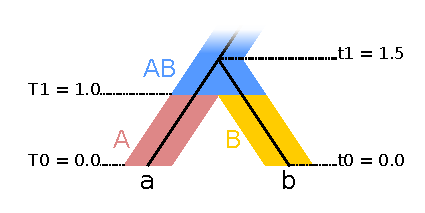
\includegraphics[width=2.5in]{relaxed_clock.pdf}
%DIFDELCMD < %%%
\DIFdelendFL \DIFaddbeginFL 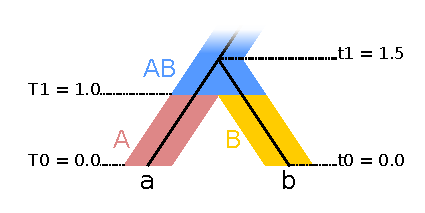
\includegraphics[width=65mm]{relaxed_clock.pdf}
\DIFaddendFL \caption
{Two-species phylogeny used to illustrate species tree relaxed
clocks. There are two extant species ``A'' and ``B'', and one ancestral species ``AB''.
Within the species tree there is a single gene tree with extant individuals ``a''
and ``b''. The single speciation event occurs at time T1, and the single coalescence
event occurs at time t1.}
\label{fig:branchRateModel}
\end{figure}

\section{Results \DIFaddbegin \DIFadd{and Discussion}\DIFaddend }

\subsection{StarBEAST2 correctly implements the multispecies coalescent}

New methods must be shown to be correct implementations of the target model.
One way to accomplish this for MCMC methods is to estimate parameters from a
prior distribution using the MCMC kernel, and to also draw independent samples
from the same distribution by simulation. The resulting parameter
distributions should be identical if the implementation is correct. We used
this method to test the correctness of the novel features in StarBEAST2;
analytical population size integration, coordinated operators, and species
tree relaxed clocks. Simulated and StarBEAST2 distributions were identical for
species and gene tree topologies (Figure~S1,S2), species and gene tree node
heights (Figure~S3,S4), and for gene tree branch rates (Figure~S5,S6). This
combination of results supports the correctness of the StarBEAST2
implementation.

\DIFaddbegin \subsection{\DIFadd{Species tree relaxed clocks prevent SPILS}}

\DIFadd{When using concatenation to infer a species tree, SPILS causes apparent
substitution rate variation among predictable species tree branches. However
in an ultrametric (time tree) framework like BEAST, branch lengths are
constrained so that terminal species begin at time zero. We hypothesized that
if a relaxed clock is used with concatenation in an ultrametric framework,
SPILS will be absorbed as faster substitution rates for lineages that would be
lengthened by SPILS in a non-ultrametric framework.
}

\DIFadd{In an ultrametric framework with a strict clock and no external (e.g. fossil,
biogeographical or known clock rate) calibrations, the substitution rate of
each branch is set to 1. This ensures that 1 unit of time is equivalent to 1
expected substitution. Using a relaxed clock with no external calibrations the
substitution rate of each branch can vary, but the expectation of the mean
rate of all branches is 1, preserving the relationship of 1 unit of time = 1
expected substitution. Therefore when SPILS causes the rates of some branches
to be faster than 1, the rates of other branches will be slower than 1 to keep
the expected mean constant.
}

\DIFadd{We used BEAST concatenation and StarBEAST2 with a species tree relaxed clock
to infer the branch lengths and substitution rates of simulated species trees
with the topology ((((A,B),C),D),E), using sequence alignments simulated using
a strict clock. Gene tree discordance will increase the estimated length of A,
B and C branches for these species trees \mbox{%DIFAUXCMD
\citep{Mendes01072016}}%DIFAUXCMD
, and as
hypothesized substitution rates for A and B branches inferred using
concatenation were biased towards being faster than the true rate of 1
(Figure~\ref{fig:spilsRates}). Estimated substitution rates for the C branch
were more variable, and could be faster or slower than 1. Substitution rates
estimated for the D and E branches were biased towards being slower than 1,
presumably to balance the mean rate. Concatenation also overestimated the
lengths of tip branches, another known bias when using concatenation to infer
a species tree \mbox{%DIFAUXCMD
\citep{Ogilvie01052016}}%DIFAUXCMD
. No biases were observed for the branch
rates or lengths estimated using StarBEAST2 (Figure~\ref{fig:spilsRates}).
}

\begin{figure*}[htb!]
\centering
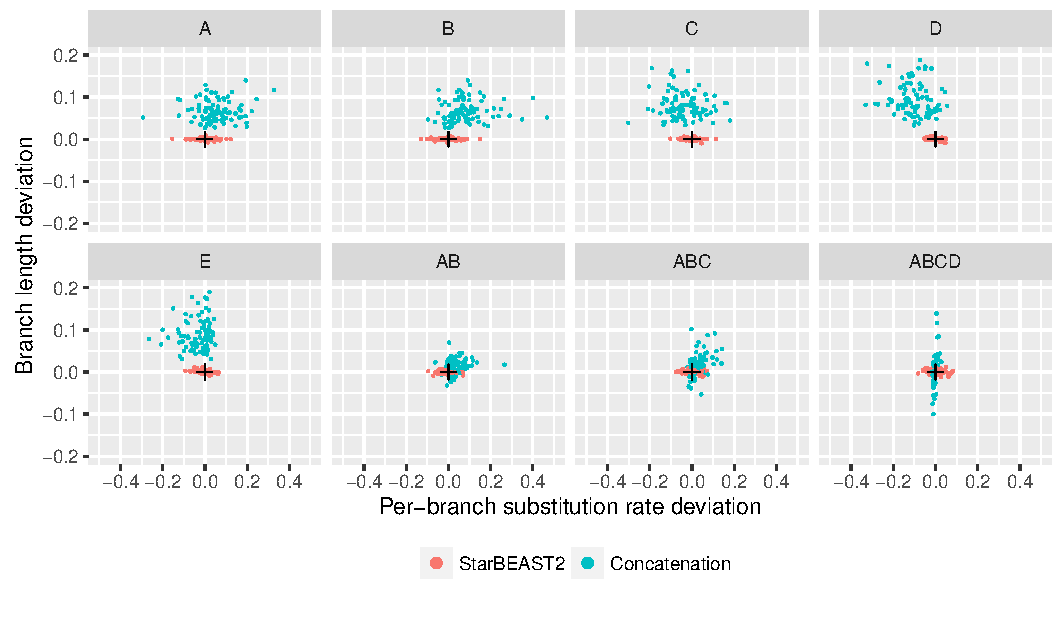
\includegraphics[width=\textwidth]{scatter.pdf}
\caption
{\DIFaddFL{Accuracy of branch substitution rates and lengths inferred by BEAST
concatenation and StarBEAST2. Deviation is the difference of each estimated
rate and length from the true value. Estimated rates and lengths are the
posterior expectation of the overall substitution rate and length for each
species tree branch. Black crosses in each panel indicate the point of perfect
accuracy. Each panel shows the distributions for the labelled extant or
ancestral branch. N = 96.}}
\label{fig:spilsRates}
\end{figure*}

\DIFadd{A number of estimated branch rates had 95\% credible intervals that excluded
the true rate of 1 when using concatenation. If a study is testing whether
substitution rates vary across a species tree, those branch rates could be
erroneously interpreted as faster or slower than average. In our simulations,
the clock rate of the D branch would be inferred as slower than average in 37
out of 96 replicates (Figure~S9), despite the sequence data being simulated
using a strict clock. When applying the same 95\% credible intervals to branch
lengths, the true simulated length was excluded with just two exceptions for
all tip branches across all replicates using concatenation (Figure~S10). In
contrast, no erroneous results would be inferred for branch rates given the
same data using StarBEAST2, and out of the 768 total simulated non-root branch
lengths, only five erroneous results would be inferred (Figure~S9,S10).
}

\DIFadd{\mbox{%DIFAUXCMD
\cite{Mendes01072016} }%DIFAUXCMD
demonstrated that SPILS causes systematic bias when
estimating branch lengths, and we show that this translates into systematic
bias when estimating per-branch substitution rates. Because the bias is caused
by incomplete lineage sorting which is a function of population sizes and
branch lengths, there is no reason to expect that large trees with varying
population sizes and branch lengths would be any less biased.
}

\DIFaddend \subsection{\textit{Pseudacris} chorus frogs have intermediate coalescent branch lengths}

To characterize the performance of coordinated operators, methods of
population size integration and relaxed clocks, we tested StarBEAST2 using
\DIFdelbegin \DIFdel{real }\DIFdelend \DIFaddbegin \DIFadd{empirical and simulated }\DIFaddend sequence data. The \DIFaddbegin \DIFadd{empirical }\DIFaddend data set used for this
analysis is from the North American chorus frog genus \textit{Pseudacris}, and
was originally collected and analyzed by \cite{Barrow201478}. \DIFaddbegin \DIFadd{This data set
has 26 nuclear locus sequences from 44 sampled individuals. The individuals
belong to 19 extant }\textit{\DIFadd{Pseudacris}} \DIFadd{lineages and two outgroup species.
\mbox{%DIFAUXCMD
\cite{Barrow201478} }%DIFAUXCMD
reported phased haplotypes but to avoid wasting
computational resources we used a single haplotype per individual.
}

\DIFaddend A key metric of phylogenies that can be used to judge whether it is necessary
to employ MSC models is the average branch length in coalescent units
$\nicefrac{\tau}{2N_e}$. \DIFaddbegin \DIFadd{In this study, $N_e$ will always refer to the
effective population size of diploid individuals. }\DIFaddend Given short branch lengths,
likelihood-based or neighbor-joining concatenation is unable to infer accurate
species trees regardless of the number of loci used, but for long branch
lengths, concatenation is approximately as accurate as *BEAST
\citep{Ogilvie01052016}. Using StarBEAST2, the average branch length within
this genus was \DIFdelbegin \DIFdel{determined to be $\nicefrac{3.22\tau}{2N_e}$}\DIFdelend \DIFaddbegin \DIFadd{estimated to be $\nicefrac{2.81\tau}{2N_e}$}\DIFaddend . This is an
intermediate average length compared to the shallow simulations analyzed by
\cite{Ogilvie01052016} which had a shorter average length of
\DIFdelbegin \DIFdel{$\nicefrac{0.54\tau}{2N_e}$}\DIFdelend \DIFaddbegin \DIFadd{$\nicefrac{1.08\tau}{2N_e}$.
}

\DIFadd{Each replicate of each }\textit{\DIFadd{Pseudacris}} \DIFadd{empirical analysis used the same
sequence data, and the true species tree topology, dates and rates were not
known with certainty. For performance results more generally applicable than a
single empirical system, and to measure the accuracy of StarBEAST2 inference,
we created a simulated data set of 30 replicates. A unique species tree was
simulated for each replicate, and gene trees and locus sequences were
simulated according to the MSC.
}

\DIFadd{We simulated 26 nuclear loci from 21 extant species with two individual
haplotypes per species, very similar to the empirical data set size. The
simulation parameters, including the birth rate, death rate and population
sizes, were also chosen to be similar to estimated }\textit{\DIFadd{Pseudacris}}
\DIFadd{parameters. The simulated data set had an average branch length of
$\nicefrac{2.99\tau}{2N_e}$, so the relative accuracy of MSC models compared
to concatenation should be comparable with empirical systems like
}\textit{\DIFadd{Pseudacris}}\DIFaddend .

\subsection{Coordinated height changing operators and analytical integration improve performance}

To determine which configuration of new features would achieve the best
performance, we ran StarBEAST2 using different combinations of operators,
methods of population size integration and \DIFdelbegin \DIFdel{different relaxed clocks}\DIFdelend \DIFaddbegin \DIFadd{clock models}\DIFaddend . To measure
convergence both effective sample size (ESS) per hour and ESS per million
states were computed for each independent chain. ESS per hour can be used to
calculate the total time required for a converged chain (nominally where ESS
equals or exceeds 200), and reflects how effectively operators explore the
space of trees and parameters, as well as the computational time required by
each operator proposal and likelihood calculation. In contrast, ESS per
million states reflects only the exploration of tree and parameter space
independently of calculation times. A variety of statistics were recorded for
each analysis (Table~S1-S4), and for each replicate the statistic with the
slowest ESS rate for that particular chain was used when computing the mean
and standard deviation of ESS per hour and per million states.

Multiple linear regressions with log transformed ESS rates as the response
variables were used to measure the effect of coordinated topology changing
operators, coordinated node height changing operators, and the method of
population size integration. Each additional feature was treated as a binary
indicator variable so that we could quantify the relative performance as a
percentage by exponentiating the coefficient for each addition
(Table~\ref{tab:convergenceLM}).
\DIFdelbegin \DIFdel{An interaction term for height changing
operators and population size integration was included because visualization of
ESS rates (Figure~\ref{fig:realEssPerHour}) suggested such an interaction existed.
}\DIFdelend 

\begin{table*}[htb!]
\caption{Relative performance of operators, population size integration and clock models.}
\label{tab:convergenceLM}
\begin{threeparttable}
\begin{tabular*}{\textwidth}{@{\extracolsep{\fill}}rlrrr@{}}
\hline
Clock model & ESS rate per & Topology\tnote{3} & Height\tnote{4} & Analytical\tnote{5}\tabularnewline
\hline
\multicolumn{5}{c}{\textit{Pseudacris} reanalysis}\tabularnewline
\hline
Strict & hour & 73\%{***} & 120\%{***} & 130\%{***}\tabularnewline
Strict & million states & 101\%\hphantom{***} & 129\%{***} & 143\%{***}\tabularnewline
GT-UCLN\tnote{1} & hour & 72\%{***} & 289\%{***} & 100\%\hphantom{***}\tabularnewline
GT-UCLN & million states & 100\%\hphantom{***} & 310\%{***} & 108\%\hphantom{***}\tabularnewline
ST-UCLN\tnote{2} & hour & 78\%{**}\hphantom{*} & 525\%{***} & 155\%{***}\tabularnewline
ST-UCLN & million states & 95\%\hphantom{***} & 511\%{***} & 164\%{***}\tabularnewline
\hline
\multicolumn{5}{c}{Simulated data}\tabularnewline
\hline
Strict & hour & 70\%{***} & 137\%{***} & 208\%{***}\tabularnewline
Strict & million states & 100\%\hphantom{***} & 148\%{***} & 225\%{***}\tabularnewline
GT-UCLN & hour & 68\%{***} & 231\%{***} & 228\%{***}\tabularnewline
GT-UCLN & million states & 98\%\hphantom{***} & 248\%{***} & 248\%{***}\tabularnewline
ST-UCLN & hour & 74\%{*}\hphantom{**} & 939\%{***} & 135\%{*}\hphantom{**}\tabularnewline
ST-UCLN & million states & 89\%\hphantom{***} & 923\%{***} & 144\%{**}\hphantom{*}\tabularnewline
\hline
\end{tabular*}
\begin{tablenotes}
\item[1] Gene Tree Uncorrelated Log-Normal relaxed clock
\item[2] Species Tree Uncorrelated Log-Normal relaxed clock
\item[3] Coordinated topology changing operators relative to na\"ive operators
\item[4] Addition of coordinated height changing operators
\item[5] Analytical integration of population sizes relative to MCMC integration
\item {*}: $p < 0.05$, {**}: $p < 0.01$, {***}: $p < 0.001$. N = 30.
\end{tablenotes}
\end{threeparttable}
\end{table*}

Coordinated topology operators \DIFdelbegin \DIFdel{had a significantly negative effect on }\DIFdelend \DIFaddbegin \DIFadd{consistently and significantly reduced }\DIFaddend ESS
per hour\DIFdelbegin \DIFdel{of gene tree relaxed clock analyses, but }\DIFdelend \DIFaddbegin \DIFadd{, but had }\DIFaddend no significant effect on ESS per million states
(Table~\ref{tab:convergenceLM}), suggesting that coordinated topology
operators are no more effective than na\"ive operators at proposing new
states. A decrease in the number of states per hour (Figure~S8) shows that
they are more computationally expensive than na\"ive operators, and explains
the negative effect on ESS per hour.

\begin{figure*}[htb!]
\centering
\DIFdelbeginFL %DIFDELCMD < 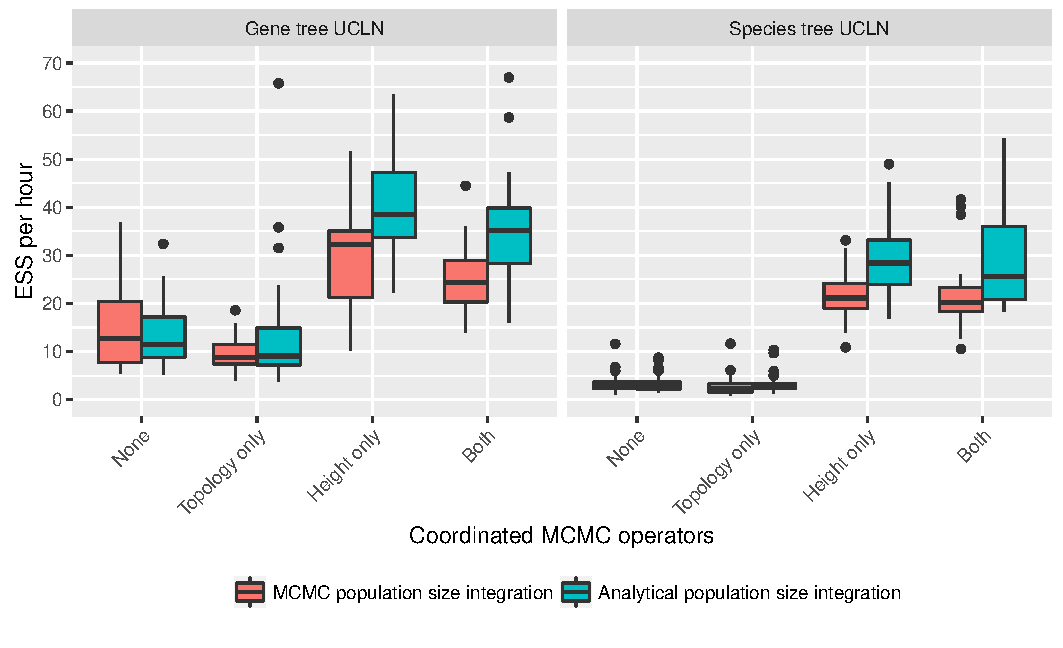
\includegraphics[width=\textwidth]{minimum_ess_per_hour_boxplot.pdf}
%DIFDELCMD < %%%
\DIFdelendFL \DIFaddbeginFL 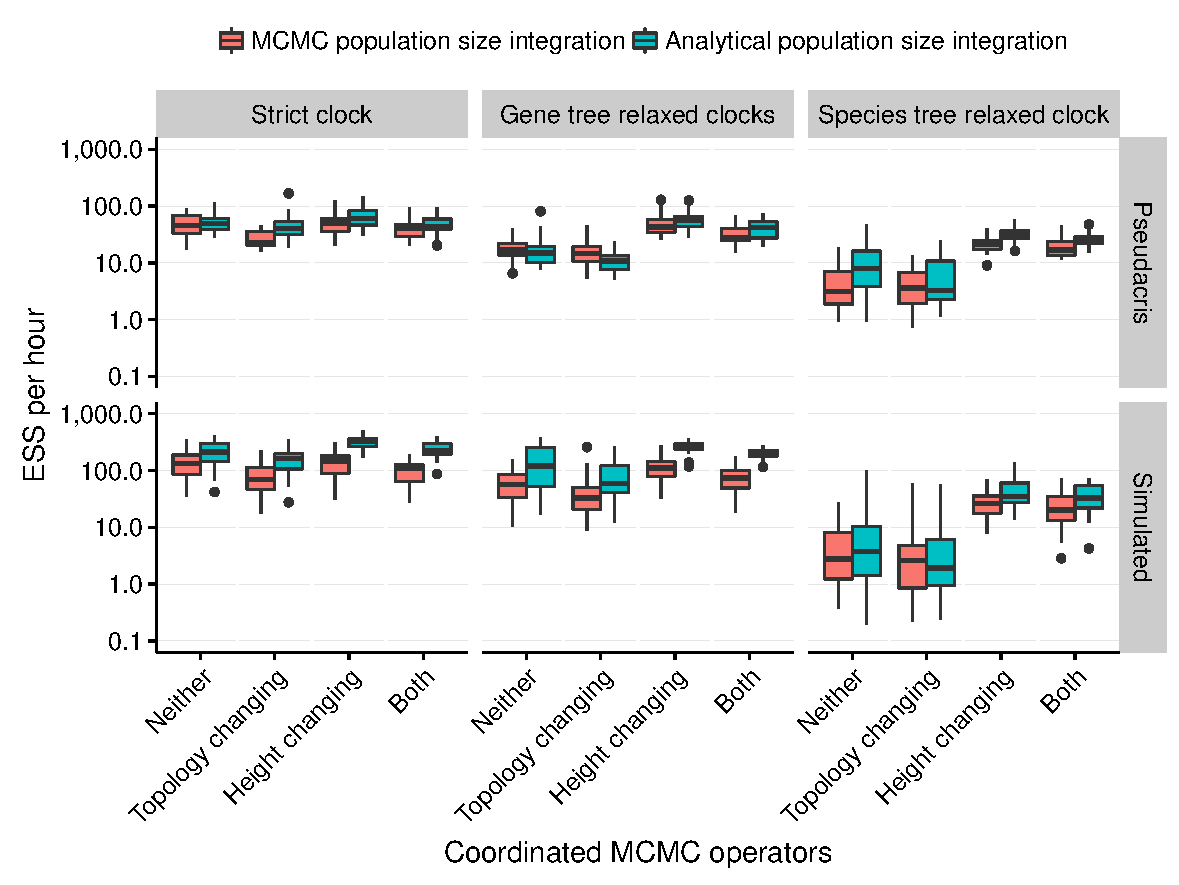
\includegraphics[width=\textwidth]{minimum_ess_per_hour_starbeast2.pdf}
\DIFaddendFL \caption
{Impact of operators, population size integration and clock models on
convergence\DIFdelbeginFL \DIFdelFL{of }\textit{\DIFdelFL{Pseudacris}} %DIFAUXCMD
\DIFdelFL{reanalyses}\DIFdelendFL . The estimated sample size (ESS) per hour for a given replicate
used the smallest ESS out of all recorded statistics. Topology refers to the
replacement of na\"ive nearest-neighbor interchange and subtree prune and
regraft operators with coordinated operators. Height refers to the addition of
operators which make coordinated changes to node heights. Uncorrelated \DIFdelbeginFL \DIFdelFL{log-normal (UCLN) }\DIFdelendFL \DIFaddbeginFL \DIFaddFL{log-
normal }\DIFaddendFL relaxed clocks were applied to either each gene tree \DIFaddbeginFL \DIFaddFL{(GT-UCLN) }\DIFaddendFL or to
the species tree \DIFaddbeginFL \DIFaddFL{(ST-UCLN)}\DIFaddendFL . N = \DIFdelbeginFL \DIFdelFL{32.}\DIFdelendFL \DIFaddbeginFL \DIFaddFL{30.}\DIFaddendFL }
\label{fig:realEssPerHour}
\end{figure*}

\DIFdelbegin \DIFdel{For gene tree and }\DIFdelend \DIFaddbegin \DIFadd{Coordinated height changing operators consistently and significantly
increased ESS per hour and ESS per million states, however the degree of
improvement depended on the clock model (Figure~\ref{fig:realEssPerHour}). For
strict clock analyses the increase in ESS per hour was modest at 1.2 times and
1.37 times for empirical and simulated data respectively, whereas for }\DIFaddend species
tree relaxed \DIFdelbegin \DIFdel{clock analyses, convergence rates
using coordinated height changing operators were 2.47 times and 7.53 times as fast respectively
than
without those operators }\DIFdelend \DIFaddbegin \DIFadd{clocks the increase was 5.25 times and 9.39 times respectively
}\DIFaddend (Table~\ref{tab:convergenceLM}). The difference \DIFdelbegin \DIFdel{made to }\DIFdelend \DIFaddbegin \DIFadd{in }\DIFaddend species tree relaxed clock
performance suggests that coordinated height changing operators are necessary
for practical implementations of that model\DIFdelbegin \DIFdel{(Figure~\ref{fig:realEssPerHour})}\DIFdelend .

\DIFdelbegin \DIFdel{Species tree relaxed clocks with coordinated height changing operators were
faster in terms of ESS per million states than gene tree relaxed clocks
(Figure~S7), showing that new state proposals are more effective. However
changing a species tree branch rate requires updating the phylogenetic
likelihood for all gene trees so the computational cost is much higher than for
gene tree relaxed clocks (Figure~S8), so species tree relaxed clocks are still
moderately slower than }\DIFdelend \DIFaddbegin \DIFadd{Analytical population size integration significantly improved ESS per hour
performance in all cases, with the exception of }\DIFaddend gene tree relaxed clocks
\DIFdelbegin \DIFdel{in terms of ESS per hour
(Figure~\ref{fig:realEssPerHour}).
}%DIFDELCMD < 

%DIFDELCMD < %%%
\DIFdel{In the absence of coordinated height changing operators, analytical population
size integration had no significant effect on performance under any
circumstance. However when combined with those operators, significant increases
}\DIFdelend \DIFaddbegin \DIFadd{applied to the }\textit{\DIFadd{Pseudacris}} \DIFadd{data set. For the simulated analyses there
was a significant improvement }\DIFaddend to ESS per hour and ESS per million states
\DIFdelbegin \DIFdel{were observed for both gene tree and
species tree relaxed clock analyses }\DIFdelend \DIFaddbegin \DIFadd{regardless of clock model }\DIFaddend (Table~\ref{tab:convergenceLM}).

\DIFdelbegin \subsection{\DIFdel{Species tree relaxed clocks prevent SPILS}}
%DIFAUXCMD
\addtocounter{subsection}{-1}%DIFAUXCMD
%DIFDELCMD < 

%DIFDELCMD < %%%
\DIFdel{When using concatenation to infer a species tree, SPILS causes apparent
substitution rate variation among predictable species tree branches. However in
an ultrametric (time tree) framework like BEAST, branch lengths are constrained so that
terminal species begin at time zero. We hypothesized that if a relaxed clock is
used with concatenation in an ultrametric framework, SPILS will be absorbed as
faster substitution rates for lineages that would be lengthened by SPILS in a
non-ultrametric framework.
}%DIFDELCMD < 

%DIFDELCMD < %%%
\DIFdel{In an ultrametric framework with a strict clock and no external (e.g. fossil,
biogeographical or known clock rate)
calibrations, the substitution rate of each branch is set to 1. This ensures that 1 unit of time
is equivalent to 1 expected substitution. Using a relaxed clock with no external calibrations
the substitution rate of each branch can vary, but the expectation of the mean rate of all
branches is 1, preserving the relationship of 1 unit of time = 1 expected substitution.
Therefore when SPILS causes the rates of some branches to be faster than 1, the rates of other branches will be slower than 1 to keep the expected mean constant.
}%DIFDELCMD < 

%DIFDELCMD < %%%
\DIFdel{We used BEAST concatenation and StarBEAST2 with a }\DIFdelend \DIFaddbegin \DIFadd{Even with new operators and analytical population size integration, the ESS
per hour rates for }\DIFaddend species tree relaxed \DIFdelbegin \DIFdel{clock to
infer the branch lengths and substitution rates of simulated species trees with
the topology ((((A,B),C),D),E), using sequence alignments simulated using a strict
clock. Gene tree discordance will increase the estimated length of A, B and C
branches for these species trees \mbox{%DIFAUXCMD
\citep{Mendes01072016}}%DIFAUXCMD
, and as hypothesized
substitution rates for A and B branches inferred using concatenation were biased
towards being faster than the true rate of 1 (Figure~\ref{fig:spilsRates}).
Estimated substitution rates for the C branch were more variable, and could be
faster or slower than 1. Substitution rates estimated for the D and E branches
were biased towards being slower than 1, presumably to balance the mean rate. Concatenation also overestimated the lengths of tip branches, another known
bias when using concatenation to infer a species tree \mbox{%DIFAUXCMD
\citep{Ogilvie01052016}}%DIFAUXCMD
. No biases were observed for the branch rates or lengths estimated using StarBEAST2
}\DIFdelend \DIFaddbegin \DIFadd{clocks were slower than for other
clock models }\DIFaddend (Figure~\DIFdelbegin \DIFdel{\ref{fig:spilsRates}). }%DIFDELCMD < 

%DIFDELCMD < \begin{figure*}[htb!]
%DIFDELCMD < \centering
%DIFDELCMD < 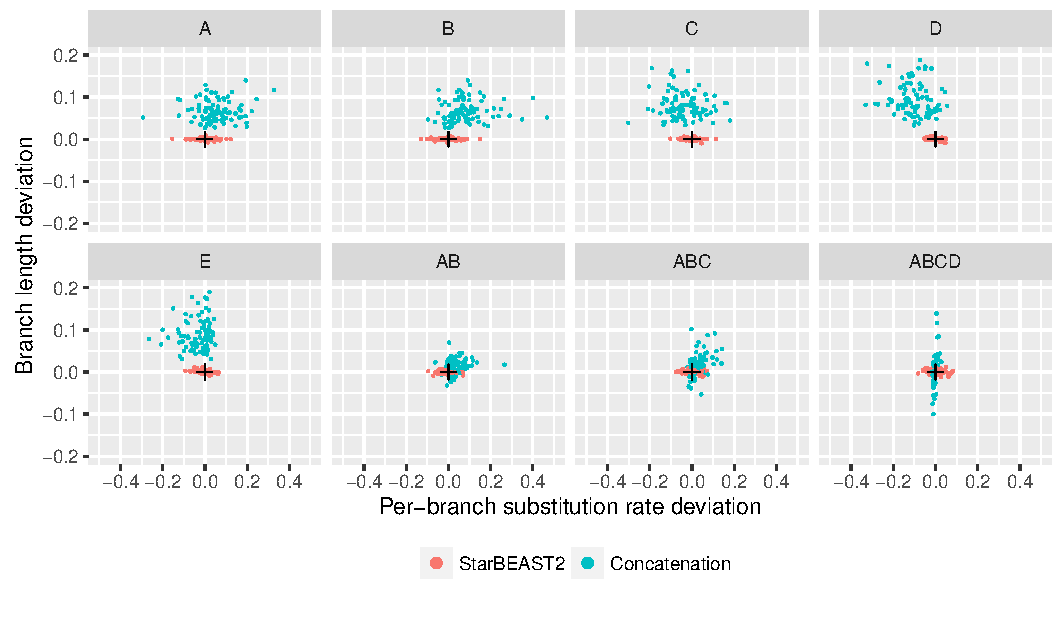
\includegraphics[width=\textwidth]{scatter.pdf}
%DIFDELCMD < \caption
%DIFDELCMD < {%%%
\DIFdelFL{Accuracy of branch substitution rates and lengths inferred by BEAST
concatenation and StarBEAST2. Deviation is the difference of each estimated
rate and length from the true value. Estimated rates and lengths are the posterior
expectation of the overall substitution rate and length for each species tree
branch. Black crosses in each panel indicate the point of perfect accuracy. Each
panel shows the distributions for the labelled extant or ancestral branch. N =
96.}%DIFDELCMD < }
%DIFDELCMD < %DIFDELCMD < \label{fig:spilsRates}%%%
%DIFDELCMD < \end{figure*}
%DIFDELCMD < 

%DIFDELCMD < %%%
\DIFdel{A number of estimated branch rates had 95\% credible intervals that excluded the
true rate of 1 when using concatenation. If a study is testing whether
substitution rates vary across }\DIFdelend \DIFaddbegin \DIFadd{\ref{fig:realEssPerHour}). One reason is that changing }\DIFaddend a
species tree \DIFdelbegin \DIFdel{, those branch rates could be
erroneously interpreted as faster or slower than average. In our simulations,
the clock rate of the D branch would be inferred as slower than average in 37
out of 96 replicates (Figure~S9), despite the sequence data being simulated
using a strict clock. When applying the same 95\% credible intervals to branch
lengths, the true simulated length was excluded with just two exceptions for all tip branches across all replicates using concatenation }\DIFdelend \DIFaddbegin \DIFadd{branch rate requires updating the phylogenetic likelihood for all
gene trees, so the computational cost is much higher than for strict or gene
tree relaxed clocks }\DIFaddend (Figure~\DIFdelbegin \DIFdel{S10).
In
contrast, no erroneous results would be inferred for branch rates given the same
data using StarBEAST2, and out of the 768 total simulated non-root branch
lengths, only five erroneous resultswould be inferred (Figure~S9, S10).
}\DIFdelend \DIFaddbegin \DIFadd{S8).
}\DIFaddend 

\DIFdelbegin \subsection{\DIFdel{StarBEAST2 is several times faster than *BEAST}}
%DIFAUXCMD
\addtocounter{subsection}{-1}%DIFAUXCMD
\DIFdelend \DIFaddbegin \subsection{\DIFadd{StarBEAST2 is an order of magnitude faster than *BEAST}}
\DIFaddend 

\DIFdelbegin \DIFdel{Our reanalysis of }\textit{\DIFdel{Pseudacris}} %DIFAUXCMD
\DIFdel{sequence data shows that }\DIFdelend \DIFaddbegin \DIFadd{StarBEAST2 also optimizes the core multispecies coalescent algorithms by
replacing recursion with loops and caching intermediate values. Operator
weights have also been tweaked by manual iteration for better performance.
Building on our results, by default StarBEAST2 enables }\DIFaddend coordinated height
changing operators \DIFdelbegin \DIFdel{,
and analytical integration of population sizes when combined with those operators, improve convergence. To show that this increased performance is generally
applicable, and to demonstrate that StarBEAST2 can accurately reconstruct
species trees, we needed to apply }\DIFdelend \DIFaddbegin \DIFadd{and analytical population size integration, but keeps
na\"ive topology operators. To measure the combined improvement when
}\DIFaddend StarBEAST2 \DIFdelbegin \DIFdel{to simulated data sets for
which the true species trees are known. To accomplish this we simulated 96 species
trees of 19 taxa each under a birth-death model with log-normally distributed
branch rates. Gene trees evolving within each species tree were simulated
according to the MSC model with log-normally distributed mean clock rates.
Finally, sequences were simulated according to an HKY process for each gene
\mbox{%DIFAUXCMD
\citep{Hasegawa1985, Goldman1993}}%DIFAUXCMD
. The parameters used for these simulations
were chosen to produce intermediate branch lengths in coalescent units; the
average simulated branch length was $\nicefrac{3.22\tau}{2N_e}$, the same as for
}\textit{\DIFdel{Pseudacris}} %DIFAUXCMD
\DIFdel{to two decimal places.
}%DIFDELCMD < 

%DIFDELCMD < %%%
\DIFdel{Simulated data was analyzed using concatenation with BEAST and using the MSC with
}\DIFdelend \DIFaddbegin \DIFadd{is applied to }\textit{\DIFadd{Pseudacris}} \DIFadd{data we compared the performance
of StarBEAST2 with default settings to *BEAST. For the simulation data set, we
compare }\DIFaddend StarBEAST2 with *BEAST \DIFdelbegin \DIFdel{settings,
high performance settings with gene tree relaxed clocks, and high performance settings with
species tree relaxed clocks.
*BEAST settings matched the configuration of *BEAST
before StarBEAST2; explicit MCMC integration of population sizes, no
coordinated operators, na\"ive NNI and SPR topology operators, and a UCLN
relaxed clock applied to each gene tree. High performance settings included analytical
integration of population sizes, coordinated height changing operators, }\DIFdelend and \DIFdelbegin \DIFdel{na\"ive NNI and SPR topology operators}\DIFdelend \DIFaddbegin \DIFadd{also concatenation.
}

\DIFadd{NGS data sets may have hundreds or thousands of loci. To gauge the performance
of StarBEAST2 applied to these data sets, we tested an empirical NGS data set;
ultraconserved element \mbox{%DIFAUXCMD
\citep[UCE;][]{Faircloth01102012} }%DIFAUXCMD
sequences from
Philippine shrews of the genus }\textit{\DIFadd{Crocidura}} \DIFadd{\mbox{%DIFAUXCMD
\citep{Giarla01092015}}%DIFAUXCMD
. This
data set consists of 1112 loci sampled from a total of 19 individuals, which
belong to 9 extant lineages}\DIFaddend . Again multiple statistics were recorded to
compute the ESS rate means and standard deviations (Table~\DIFdelbegin \DIFdel{S5-S8}\DIFdelend \DIFaddbegin \DIFadd{SXXX-SXXX}\DIFaddend ).

Our simulation study confirmed that StarBEAST2 is \DIFdelbegin \DIFdel{several }\DIFdelend \DIFaddbegin \DIFadd{many }\DIFaddend times faster than
*BEAST (Figure~\DIFdelbegin \DIFdel{\ref{fig:simulatedEssPerHour}}\DIFdelend \DIFaddbegin \DIFadd{\ref{fig:essPerHourComparison}}\DIFaddend ). For simulated data the average
log convergence rate of StarBEAST2 with \DIFdelbegin \DIFdel{high performance settings and }\DIFdelend gene tree relaxed clocks was \DIFdelbegin \DIFdel{4.01 }\DIFdelend \DIFaddbegin \DIFadd{5.54
}\DIFaddend $\ln(\nicefrac{ESS}{hour})$. This compares to \DIFdelbegin \DIFdel{2.18 }\DIFdelend \DIFaddbegin \DIFadd{2.04 }\DIFaddend using *BEAST settings, an
increase in performance of \DIFdelbegin \DIFdel{$\exp(4.01 - 2.18) = 6.2$ }\DIFdelend \DIFaddbegin \DIFadd{$\exp(5.54 - 2.04) = 33.1$ }\DIFaddend times (Table~S5). \DIFdelbegin \DIFdel{However
for }\textit{\DIFdel{Pseudacris}} %DIFAUXCMD
\DIFdel{reanalyses the average was
3.66 for StarBEAST2 compared
to 2.52 for }\DIFdelend \DIFaddbegin \DIFadd{Even
when using 52 loci --- twice as many as used with }\DIFaddend *BEAST \DIFdelbegin \DIFdel{, a smaller increase of 3.1 }\DIFdelend \DIFaddbegin \DIFadd{--- StarBEAST2 was
$\exp(4.18 - 2.04) = 8.5$ times faster.
}

\DIFadd{StarBEAST2 was still an order of magnitude faster when analyzing either
empirical data set. For gene tree relaxed clock reanalyses of
}\textit{\DIFadd{Pseudacris}} \DIFadd{the difference was $\exp(3.98 - 1.42) = 13.0$ times. For
50-locus }\textit{\DIFadd{Crocidura}} \DIFadd{reanalyses it was $\exp(2.79 - 0.11) = 14.6$ }\DIFaddend times
(Table~S1). \DIFaddbegin \DIFadd{After doubling the number of loci to 100, StarBEAST2 was still
faster than *BEAST with 50 loci by $\exp(0.52 - 0.11) = 1.5$ times.
}\DIFaddend 

\DIFdelbegin \DIFdel{Species }\DIFdelend \DIFaddbegin \DIFadd{The ESS per hour convergence of species }\DIFaddend tree relaxed clocks \DIFdelbegin \DIFdel{were slower than the }\DIFdelend \DIFaddbegin \DIFadd{was lower than for
}\DIFaddend gene tree relaxed clocks\DIFdelbegin \DIFdel{when
using high performance settings (Figure~\ref{fig:simulatedEssPerHour}). The
average log rate for simulated data when using a species tree relaxed clock with
high performance settings was 3.74, which is still 4.8 }\DIFdelend \DIFaddbegin \DIFadd{. For simulated data gene tree relaxed clocks were
$\exp(5.54 - 3.71) = 6.2$ }\DIFaddend times faster than using gene tree relaxed clocks
with *BEAST \DIFdelbegin \DIFdel{settings }\DIFdelend (Table~S5). \DIFdelbegin \DIFdel{Again the
difference was smaller for }\DIFdelend \DIFaddbegin \DIFadd{The difference was much smaller for empirical data;
for }\DIFaddend \textit{Pseudacris} reanalyses \DIFdelbegin \DIFdel{, with a rate of 3.36
for StarBEAST2, or 2.3 times faster(Table~S1).
}%DIFDELCMD < 

%DIFDELCMD < %%%
\DIFdel{The computational performance of StarBEAST2 was also more consistent than
*BEAST. The standard deviations of the log rate }\DIFdelend \DIFaddbegin \DIFadd{gene tree relaxed clocks were $\exp(3.98 -
3.44) = 1.7$ times faster, and for }\textit{\DIFadd{Crocidura}} \DIFadd{they were $\exp(2.79 -
2.12) = 2.0$ times faster. In all three cases species tree relaxed clocks
}\DIFaddend using StarBEAST2 \DIFdelbegin \DIFdel{to analyze
simulated data sets were 0.44 and 0.46 for gene and species }\DIFdelend \DIFaddbegin \DIFadd{were still faster than gene }\DIFaddend tree relaxed clocks \DIFdelbegin \DIFdel{respectively, compared to 0.73 for }\DIFdelend \DIFaddbegin \DIFadd{using }\DIFaddend *BEAST
(\DIFdelbegin \DIFdel{Table~S7).
The standard deviations
when reanalyzing }\textit{\DIFdel{Pseudacris}} %DIFAUXCMD
\DIFdel{were 0.23, 0.26 and 0.55 for StarBEAST2
with gene tree relaxed clocks, }\DIFdelend \DIFaddbegin \DIFadd{Figure~\ref{fig:essPerHourComparison}).
}

\DIFadd{The ESS per hour of concatenation with 26 loci was similar to }\DIFaddend StarBEAST2\DIFdelbegin \DIFdel{with species tree relaxed clocks, and }\DIFdelend \DIFaddbegin \DIFadd{.
However concatenation scales better than }\DIFaddend *BEAST \DIFdelbegin \DIFdel{respectively. The higher spread for simulated data reflects the fact that
each replicate used a different species tree with different genes and sequence
alignments.
}%DIFDELCMD < 

%DIFDELCMD < %%%
\DIFdel{Concatenation with the same }\DIFdelend \DIFaddbegin \DIFadd{or StarBEAST2, and we were
able to quintuple the number of loci compared to doubling the }\DIFaddend number of loci
\DIFdelbegin \DIFdel{is much faster than StarBEAST2, but
concatenation using 220 loci was similar to *BEAST and slower than }\DIFdelend \DIFaddbegin \DIFadd{by using }\DIFaddend StarBEAST2\DIFdelbegin \DIFdel{(Figure~\ref{fig:simulatedEssPerHour})}\DIFdelend .

\DIFdelbegin %DIFDELCMD < \begin{figure}[htb!]
%DIFDELCMD < %%%
\DIFdelendFL \DIFaddbeginFL \begin{figure*}[htb!]
\DIFaddendFL \centering
\DIFdelbeginFL %DIFDELCMD < 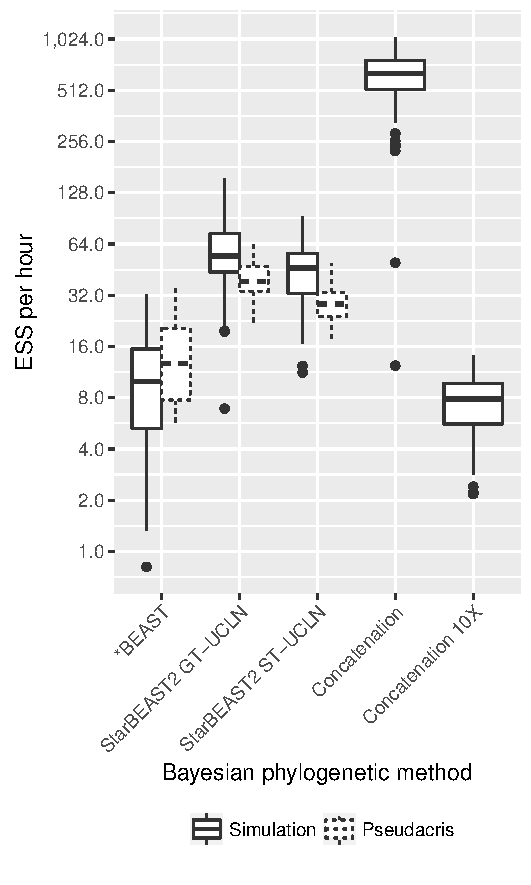
\includegraphics[width=2.5in]{combined_ess_per_hour.pdf}
%DIFDELCMD < %%%
\DIFdelendFL \DIFaddbeginFL 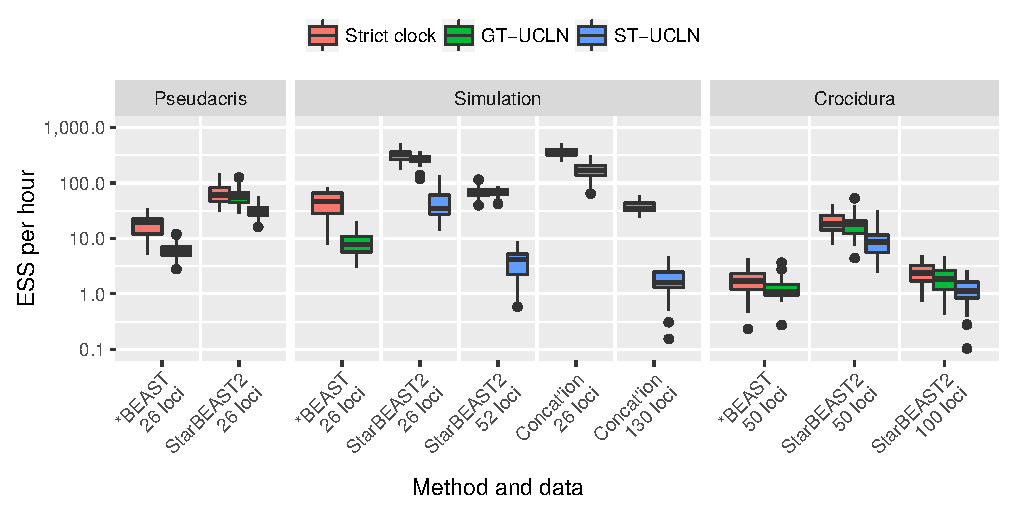
\includegraphics[width=\textwidth]{minimum_ess_per_hour_comparison.pdf}
\DIFaddendFL \caption
{Convergence of different methods applied to simulated and empirical data
sets. The estimated sample size (ESS) per hour for a given replicate used the
\DIFdelbeginFL \DIFdelFL{smallest ESS }\DIFdelendFL \DIFaddbeginFL \DIFaddFL{slowest ESS rate }\DIFaddendFL out of all recorded statistics. Methods are BEAST
concatenation\DIFdelbeginFL \DIFdelFL{with 22 loci, concatenation with 220 loci (10X), StarBEAST2 with
}\DIFdelendFL \DIFaddbeginFL \DIFaddFL{, }\DIFaddendFL *BEAST\DIFdelbeginFL \DIFdelFL{settings and 22 loci}\DIFdelendFL , and StarBEAST2 with \DIFdelbeginFL \DIFdelFL{high performance settings, 22 loci,
and }\DIFdelendFL uncorrelated log-normal relaxed
clocks applied to the gene trees (GT-UCLN) or to the species tree (ST-UCLN).
\DIFdelbeginFL \textit{\DIFdelFL{Pseudacris}} %DIFAUXCMD
\DIFdelFL{results from Figure~\ref{fig:realEssPerHour} are also reproduced for
multispecies coalescent analyses (dashed-line boxes). }\DIFdelendFL N = \DIFdelbeginFL \DIFdelFL{96 (simulated), N = 32
(}\textit{\DIFdelFL{Pseudacris}}%DIFAUXCMD
\DIFdelFL{).
}\DIFdelendFL \DIFaddbeginFL \DIFaddFL{30.}\DIFaddendFL }
\DIFdelbeginFL %DIFDELCMD < %DIFDELCMD < \label{fig:simulatedEssPerHour}%%%
%DIFDELCMD < \end{figure}
%DIFDELCMD < %%%
\DIFdelend \DIFaddbegin \label{fig:essPerHourComparison}
\end{figure*}

\DIFadd{The increased performance of StarBEAST2 will enable researchers to analyze
sequence data more quickly and disseminate their findings sooner; a large MCMC
analysis which would currently take three months may now be performed in one
week. In the case of phylogenomic data which has been subsetted for use with
*BEAST, StarBEAST2 can alternatively be used to analyze more data for more
precise estimates of species trees and other parameters in the same amount of
time as a more limited *BEAST analysis.
}\DIFaddend 

\subsection{Concatenation is a worse estimator of branch lengths than topology}

The accuracy of StarBEAST2 relative to BEAST concatenation varied depending on
the type of error and whether equal numbers of loci were used. Relative
species tree error measures the accuracy of estimated branch lengths; by that
measure StarBEAST2 using \DIFdelbegin \DIFdel{22 }\DIFdelend \DIFaddbegin \DIFadd{just 26 }\DIFaddend loci outperformed concatenation using \DIFdelbegin \DIFdel{22 }\DIFdelend \DIFaddbegin \DIFadd{130
}\DIFaddend loci, and \DIFdelbegin \DIFdel{matched
the performance of concatenation using 220 }\DIFdelend \DIFaddbegin \DIFadd{was even more accurate when using 52 }\DIFaddend loci
(Figure~\ref{fig:speciesTreeError}A). Pendant edge bias measures systematic
bias in the estimated ages of extant species; \DIFdelbegin \DIFdel{by that measure }\DIFdelend \DIFaddbegin \DIFadd{regardless of the number of loci
}\DIFaddend StarBEAST2 was much less biased \DIFdelbegin \DIFdel{even when concatenation was used with ten-fold more data
}\DIFdelend \DIFaddbegin \DIFadd{than concatenation which overestimated tip
branch lengths by about 250\% }\DIFaddend (Figure~\ref{fig:speciesTreeError}B). \DIFaddbegin \DIFadd{This is
less than the 350\% reported in \mbox{%DIFAUXCMD
\cite{Ogilvie01052016} }%DIFAUXCMD
because of longer
average branch lengths in coalescent units in this study.
}

\DIFadd{Pendant edge bias is important because many published phylogenies show
evidence of a slowdown in diversification rate \mbox{%DIFAUXCMD
\citep{Moen2014190}}%DIFAUXCMD
. If the
ages of extant species are overestimated, this will artificially reduce the
number of recent speciation events, mimicking a slowdown. We suggest that
accurate inference of changing diversification rates requires species trees
inferred by fully Bayesian MSC methods like StarBEAST2.
}

\DIFaddend Rooted Robinson-Foulds distance measures the topological accuracy of estimated
trees; for that metric concatenation using \DIFdelbegin \DIFdel{22 loci was almost as accurate as }\DIFdelend \DIFaddbegin \DIFadd{130 loci was similar in accuracy to
}\DIFaddend StarBEAST2 \DIFdelbegin \DIFdel{, and more accurate when using 220 }\DIFdelend \DIFaddbegin \DIFadd{using 52 }\DIFaddend loci (Figure~\ref{fig:speciesTreeError}C). \DIFaddbegin \DIFadd{When the number
of loci was the same, StarBEAST2 outperformed concatenation. }\DIFaddend For no type of
error did the choice of gene or species tree relaxed clocks significantly
affect the accuracy of StarBEAST2 (Figure~\ref{fig:speciesTreeError}A,B,C).

\DIFaddbegin \DIFadd{Using unphased sequences with ambiguity codes for heterozygous sites improved
the accuracy of concatenation by reducing the pendant edge bias from about
250\% to about 50\% (Figure~SXXX). Ambiguity codes are treated by most
phylogenetic methods (including BEAST concatenation) as base call errors,
indicating the nucleotide at a given site could be one of several
possibilities. When used with unphased sequences, they actually indicate the
presence of two nucleotides simultaneously, which is therefore a model violation.
Using concatenation to analyze unlinked loci is also a model violation, but in
the region of parameter space investigated by this simulation study the two
errors may }\textit{\DIFadd{partially}} \DIFadd{cancel out.
}

\DIFaddend \begin{figure}[htb!]
\centering
\DIFdelbeginFL %DIFDELCMD < 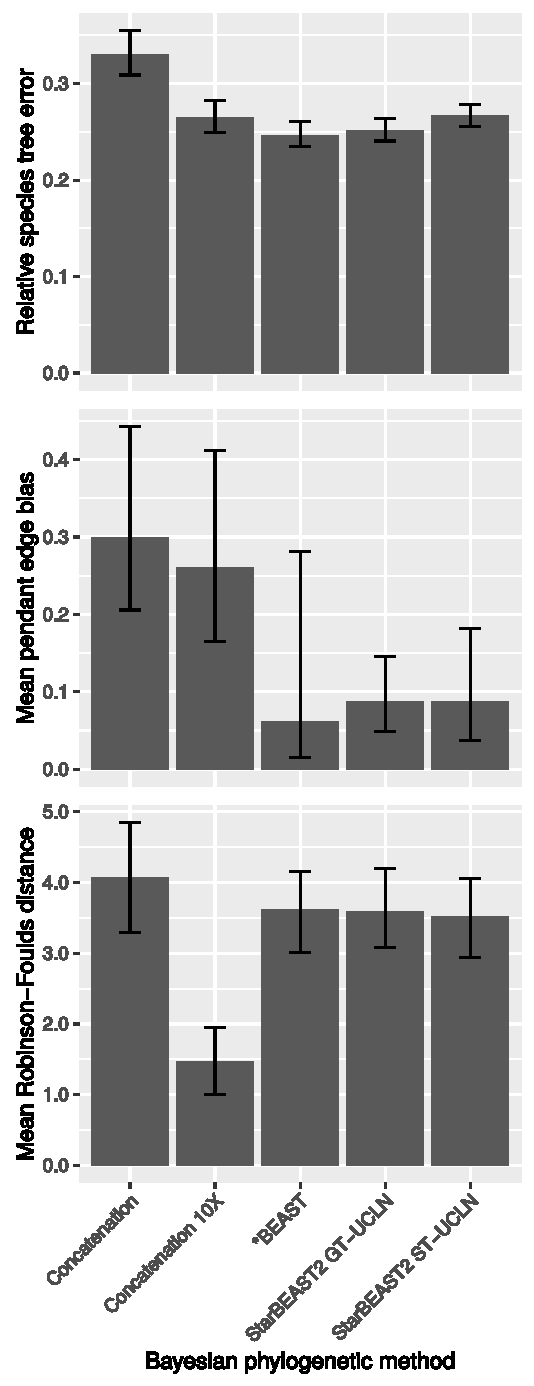
\includegraphics[width=2.5in]{tree_error.pdf}
%DIFDELCMD < %%%
\DIFdelendFL \DIFaddbeginFL 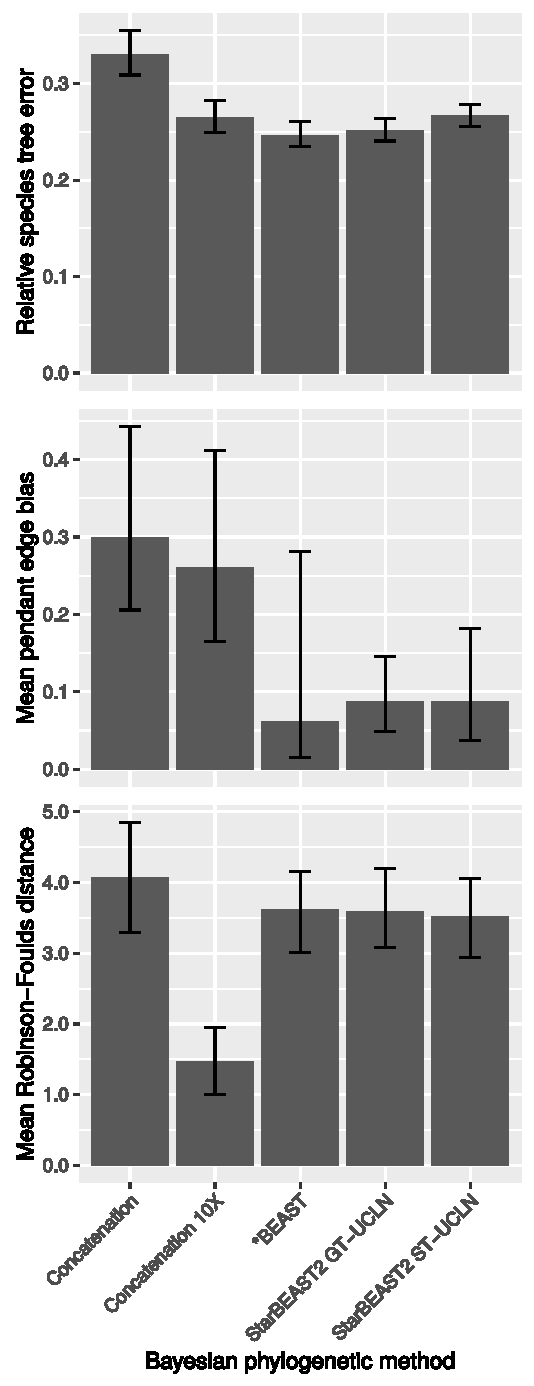
\includegraphics[width=65mm]{tree_error.pdf}
\DIFaddendFL \caption
{Accuracy of different methods applied to simulated data. Methods are \DIFdelbeginFL \DIFdelFL{BEAST concatenation with 22 loci, concatenation with 220 loci
(10X), }\DIFdelendFL StarBEAST2\DIFdelbeginFL \DIFdelFL{with *BEAST settings and 22 loci,
and StarBEAST2 with high performance settings, 22 loci, and }\DIFdelendFL \DIFaddbeginFL \DIFaddFL{,
*BEAST and BEAST concatenation with }\DIFaddendFL uncorrelated log-normal relaxed clocks applied
to the gene tree (GT-UCLN) or to the species tree (ST-UCLN). (A) Trimmed mean of
relative species tree error, a measure of branch length error. (B) Trimmed
mean of mean pendant edge bias, which measures biased estimates of the ages of
extant species. (C) Trimmed mean of mean rooted Robinson-Foulds (RF) distances, a
measure of topological error. 25\% trim was used to reduce the
influence of outliers. All error bars are 95\% confidence intervals calculated
by bootstrapping. N = \DIFdelbeginFL \DIFdelFL{96.}\DIFdelendFL \DIFaddbeginFL \DIFaddFL{30.}\DIFaddendFL }
\label{fig:speciesTreeError}
\end{figure}

\subsection{StarBEAST2 is superior at inferring substitution rates\DIFdelbegin \DIFdel{given intermediate branch lengths}\DIFdelend }

While the convergence of species tree relaxed clock analyses \DIFdelbegin \DIFdel{was slower }\DIFdelend \DIFaddbegin \DIFadd{took longer }\DIFaddend than
for gene tree relaxed clocks \DIFdelbegin \DIFdel{using high performance settings}\DIFdelend \DIFaddbegin \DIFadd{in StarBEAST2}\DIFaddend , species tree relaxed clocks enable
inference of species branch rates within an MSC framework. To gauge the
accuracy of estimated branch rates, we used simple linear regressions with the
true rate of each simulated branch as the explanatory variable, and the
posterior expectation of the rate of that branch (conditional on the
corresponding clade being monophyletic in the posterior samples) as the
response variable. If all estimates are equally proportional to the truth,
then the $R^2$ coefficient of determination will equal 1. \DIFaddbegin \DIFadd{There are intrinsic
limits to our ability to estimate substitution rates, primarily that branch
length is confounded with substitution rate \mbox{%DIFAUXCMD
\citep{Thorne01092002}}%DIFAUXCMD
.
}\DIFaddend 

\DIFdelbegin \DIFdel{When estimating branch ratesusing BEAST concatenation with either 22 or 220 loci ,
}\DIFdelend \DIFaddbegin \DIFadd{For analyses of simulated data using 26 loci the }\DIFaddend $R^2$ \DIFaddbegin \DIFadd{using StarBEAST2 was
$0.39$ and by doubling the number of loci to 52 was increased to $0.44$. In
contrast the $R^2$ when using concatenation with 26 }\DIFaddend was \DIFdelbegin \DIFdel{very weak at $0.07$ and $0.09$ respectively. By applying a relaxed
clock to the species tree using StarBEAST2, the $R^2$ was much higher at $0.21$
using just 22 }\DIFdelend \DIFaddbegin \DIFadd{$0.26$ and even after
increasing the number of loci to 130 it was only $0.32$, in either case worse
than StarBEAST2 using 26 }\DIFaddend loci (Figure~\ref{fig:branchRates}). \DIFaddbegin \DIFadd{StarBEAST2 is
clearly superior to concatenation at inferring branch rates, possibly even
more so than for branch lengths and topology.
}\DIFaddend 

\DIFdelbegin \DIFdel{The true standard deviation used to simulate branch rateswas 0.16, and the
estimated standard
deviation for 220 locus BEAST concatenation analyses was 0.14. In contrast the
estimated standard deviations for 22 locus analyses were 0.08 }\DIFdelend \DIFaddbegin \DIFadd{Concatenation is an even worse estimator of branch rates when using unphased
sequences with ambiguity codes for heterozygous sites (Figure~SXXX). When
applying concatenation to either 26 or 130 loci, $R^2$ was very weak at $0.12$ }\DIFaddend and
\DIFdelbegin \DIFdel{0.07 for concatenation and StarBEAST2 respectively.
This is because when the sequence
alignments are less informative for a given branch (as happens when fewer loci are
used), the posterior expectation of the rate will be close to the prior
expectation which is 1. This is evident in Figure~\ref{fig:branchRates} as the
large number of branch rates around 1 for both 22 locus analyses}\DIFdelend \DIFaddbegin \DIFadd{$0.15$ respectively (Figure~SXXX)}\DIFaddend .

\begin{figure}[htb!]
\centering
\DIFdelbeginFL %DIFDELCMD < 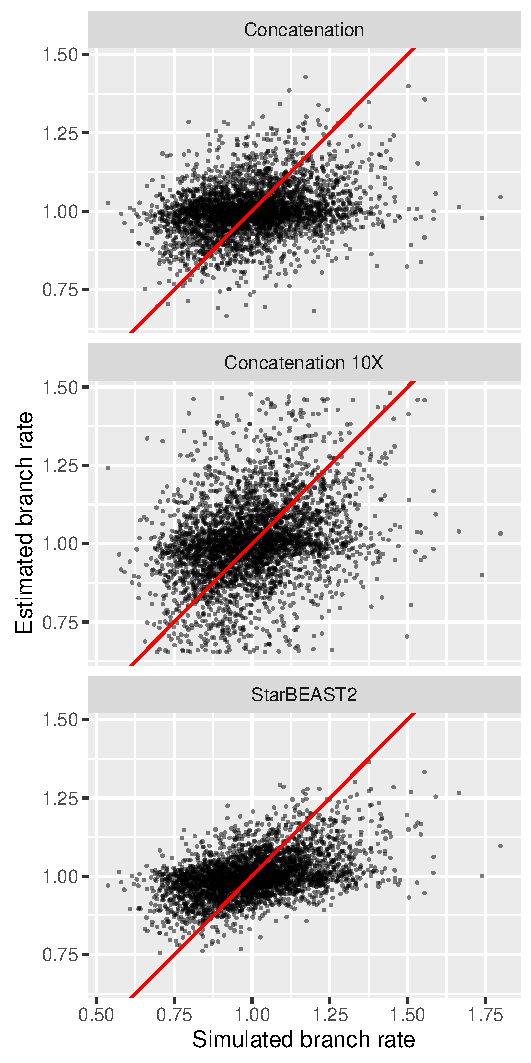
\includegraphics[width=2.5in]{branch_rates.pdf}
%DIFDELCMD < %%%
\DIFdelendFL \DIFaddbeginFL 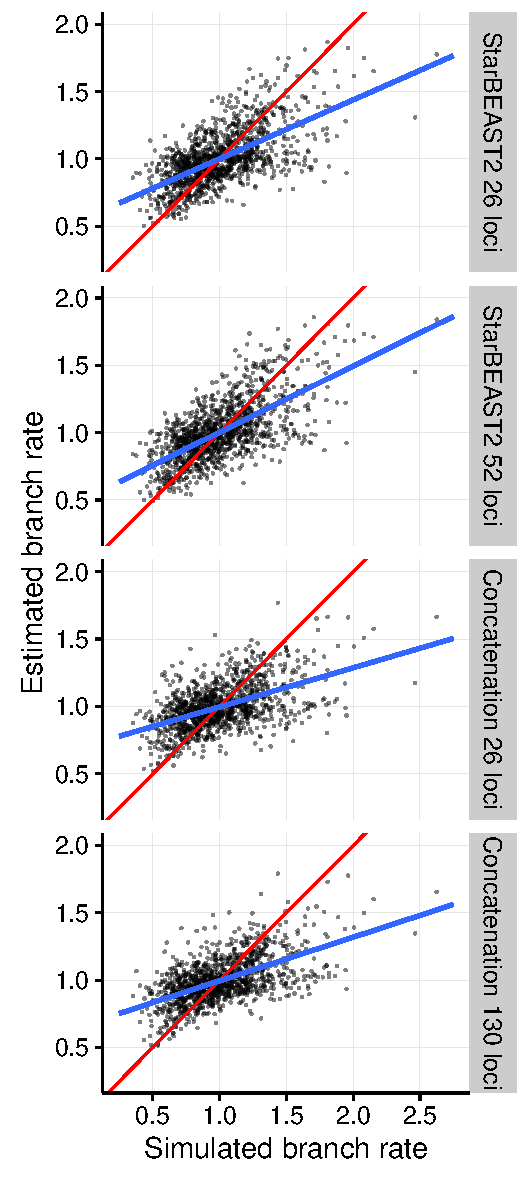
\includegraphics[width=65mm]{branch_rates_phased.pdf}
\DIFaddendFL \caption
{Estimates of species tree branch rates using BEAST concatenation versus
StarBEAST2. \DIFdelbeginFL \DIFdelFL{Methods are concatenation with 22 loci, concatenation with 220 loci (10X), and
StarBEAST2 with high performance settings, 22 loci, and a relaxed clock applied
to the species tree. }\DIFdelendFL Estimated rates are the posterior expectations of each branch rate
from each replicate. Root branch rates, which were fixed at 1, were excluded.
In blue are simple linear regression lines of best fit\DIFdelbeginFL \DIFdelFL{. N }\DIFdelendFL \DIFaddbeginFL \DIFaddFL{, and in red are the $y
= x$ lines showing a perfect relationship between estimates and truth. N }\DIFaddendFL =
\DIFdelbeginFL \DIFdelFL{96.}\DIFdelendFL \DIFaddbeginFL \DIFaddFL{30.}\DIFaddendFL }
\label{fig:branchRates}
\end{figure}

\DIFdelbegin \section{\DIFdel{Discussion}}
%DIFAUXCMD
\addtocounter{section}{-1}%DIFAUXCMD
%DIFDELCMD < 

%DIFDELCMD < %%%
\subsection{\DIFdel{StarBEAST2 will enable faster and more precise inference}}
%DIFAUXCMD
\addtocounter{subsection}{-1}%DIFAUXCMD
%DIFDELCMD < 

%DIFDELCMD < %%%
\DIFdel{The increased performance of StarBEAST2 will enable researchers to analyze
sequence data more quickly and disseminate their findings sooner; a large MCMC
analysis which would currently take six weeks might now be performed in one or two
weeks. In the case of phylogenomic data which has been subsetted for use with
*BEAST, StarBEAST2 can alternatively be used to analyze more data for more
precise estimates of species trees and other parameters in the same amount of
time as a more limited *BEAST analysis.
}%DIFDELCMD < 

%DIFDELCMD < %%%
\DIFdel{Our results show that convergence rate of different MCMC chains will vary
despite an identical StarBEAST2 configuration and data, as variation in ESS per
hour exists between replicate }\textit{\DIFdel{Pseudacris}} %DIFAUXCMD
\DIFdel{runs. The
higher standard deviation for the log ESS rate of simulation replicates suggests
that additional variation comes from the particular data set being analyzed,
because each replicate used a different species tree with different genes and
sequence alignments. The }\textit{\DIFdel{Pseudacris}} %DIFAUXCMD
\DIFdel{species tree or choice of genes to
sample may
represent a slower than average data set, as StarBEAST2 was on average 6.2 times
faster than *BEAST across the simulated data sets, compared to 3.1 times faster
for }\textit{\DIFdel{Pseudacris}}%DIFAUXCMD
\DIFdel{.
}%DIFDELCMD < 

%DIFDELCMD < %%%
\DIFdel{Previous research on the scaling behaviour of *BEAST has shown that the
relationship between the number of loci in a given analysis and the convergence
in terms of ESS per hour follows a power law based on the
the number of loci with a coefficient of approximately $-2.8$ \mbox{%DIFAUXCMD
\citep{Ogilvie01052016}}%DIFAUXCMD
. If the number of loci for a
given analysis is doubled, the convergence rate is therefore
expected to be $\exp(-2.8 \cdot \ln(2)) = 0.144 \approx \nicefrac{1}{7}$ that
of the original analysis. Based on our simulation results, this suggests that
StarBEAST2 should be able to analyze datasets of approximately twice the size
that *BEAST can in the same time.
}%DIFDELCMD < 

%DIFDELCMD < %%%
\subsection{\DIFdel{Concatenation can still be inferior given intermediate branch lengths}}
%DIFAUXCMD
\addtocounter{subsection}{-1}%DIFAUXCMD
%DIFDELCMD < 

%DIFDELCMD < %%%
\DIFdel{Likelihood-based or neighbor-joining concatenation cannot accurately
estimate branch lengths in substitutions when branches have short lengths in coalescent units.
*BEAST using just four loci can be more accurate than
concatenation using 4096 loci in terms of relative species tree error and
pendant edge bias. *BEAST can also be more accurate at estimating species tree
topologies given the same number of loci as concatenation, but inferior when
concatenation can be used with a much greater number of loci
\mbox{%DIFAUXCMD
\citep{Ogilvie01052016}}%DIFAUXCMD
.
}%DIFDELCMD < 

%DIFDELCMD < %%%
\DIFdel{We have shown that concatenation can still be inferior to *BEAST and StarBEAST2
given intermediate branch lengths. For the same number of loci, a higher
relative species tree error indicates that concatenation is less accurate at
estimating branch lengths, and a large pendant edge bias indicates that
it also tends to overestimate tip branch lengths --- equivalent to the
ages of extant species given complete species sampling. Unlike the short branch
length case, concatenation with 10 times more loci can match the multispecies
coalescent in
terms of relative species tree error, but is then slower than StarBEAST2 with
high performance settings. In other words, for intermediate branch lengths
StarBEAST2 can be just as accurate as concatenation but needs less investment in
both sequencing and computational time.
}%DIFDELCMD < 

%DIFDELCMD < %%%
\DIFdel{Concatenation does not perform as well as StarBEAST2 in terms of pendant edge bias
even using ten-fold as much data.
Pendant edge bias is important because many published phylogenies show evidence
of a slowdown in diversification rate \mbox{%DIFAUXCMD
\citep{Moen2014190}}%DIFAUXCMD
. If the ages of extant
species are overestimated, this will artificially reduce the number of recent
speciation events, mimicking a slowdown. We suggest that accurate inference of
changing diversification rates requires species trees inferred by fully Bayesian MSC methods
like StarBEAST2.
}%DIFDELCMD < 

%DIFDELCMD < %%%
\subsection{\DIFdel{The multispecies coalescent should be used to infer per-species substitution rates}}
%DIFAUXCMD
\addtocounter{subsection}{-1}%DIFAUXCMD
%DIFDELCMD < 

%DIFDELCMD < %%%
\DIFdel{Concatenation is already known to have difficulty inferring branch lengths
because of SPILS. When a gene tree contains a branch absent from the species
tree, substitutions along that branch must be attributed to multiple species tree
branches in a concatenation analysis, lengthening those branch estimates . Conversely,
when a species tree contains a branch absent from a gene tree, no substitutions
can be attributed to that branch, which will be inferred to be shorter \mbox{%DIFAUXCMD
\citep{Mendes01072016}}%DIFAUXCMD
.
We show that by using BEAST concatenation with a relaxed
clock, the estimated substitution rate of branches lengthened by
SPILS can be increased, and estimated substitution rate of other
branches can be decreased. This causes erroneous results when asking if substitution rates
are constant across a species tree. In contrast, StarBEAST2 is resistant to
SPILS and did not produce any biased estimates.
}%DIFDELCMD < 

%DIFDELCMD < %%%
\DIFdel{When given intermediate branch lengths, concatenation was unable to accurately
estimate per-species substitution rates even when using 220 loci, and it is
reasonable to assume that shorter coalescent branch lengths would
exacerbate the problem. StarBEAST2 can recover many branch rates, and given a
more informative data set than our simulation study of 22$\times$400nt loci
should be able to further improve the accuracy of estimated rates to a point.
There are intrinsic limits to our ability to estimate substitution rates,
primarily that branch length is confounded with substitution rate
\mbox{%DIFAUXCMD
\citep{Thorne01092002}}%DIFAUXCMD
. }%DIFDELCMD < 

%DIFDELCMD < %%%
\DIFdelend \section{Conclusions}

When estimating dates and rates, the choice is often between using a subset of
available loci with a fully Bayesian MSC method, or all available loci with
concatenation. Researchers have often opted for the second choice, but we have
shown that concatenation may not accurately estimate the ages of extant species
or per-species substitution rates, even for trees of intermediate branch lengths. The
increased performance of StarBEAST2 should further encourage the adoption of
fully Bayesian MSC methods for estimating divergence times, and the new species
tree relaxed clock will enable accurate inference of species branch rates despite
ILS. StarBEAST2 is free and open source software, and its source code and
development history is available through GitHub
(\url{https://github.com/genomescale/starbeast2}).

\section{Materials and Methods}

For all StarBEAST2\DIFdelbegin \DIFdel{and BEAST }\DIFdelend \DIFaddbegin \DIFadd{, *BEAST and }\DIFaddend concatenation analyses, the version of BEAST
used was 2.4\DIFdelbegin \DIFdel{.1}\DIFdelend \DIFaddbegin \DIFadd{.4}\DIFaddend . For all simulations, the version of biopy \citep{biopy} used
was 0.1.9.

\subsection{Mathematical correctness of StarBEAST2}

Simulated trees were generated using biopy, and trees sampled from a prior
distribution were generated using StarBEAST2 with all new features enabled.
This included analytical integration of population sizes, coordinated tree
topology and node height changing operators, and a species tree relaxed clock.
100,000 species trees were simulated, \DIFaddbegin \DIFadd{one gene tree was simulated per species
tree with a rate of 0.5, and a second gene tree was simulated per species tree
with a rate of 2.0.
}

\DIFadd{100,000 species trees, 100,000 half rate gene trees }\DIFaddend and 100,000 \DIFaddbegin \DIFadd{double rate
gene }\DIFaddend trees were sampled from the prior at a rate of one every 1000 after a
10\% burn-in period.

Identical parameters were used for the simulation and for the StarBEAST2 run
including the prior distributions. \DIFdelbegin \DIFdel{The
}\DIFdelend \DIFaddbegin \DIFadd{We fixed the }\DIFaddend number of species \DIFdelbegin \DIFdel{and haplotypes were fixed }\DIFdelend at 5 and \DIFdelbegin \DIFdel{1 respectively.
}\DIFdelend \DIFaddbegin \DIFadd{the
number of haplotypes per species at 1. }\DIFaddend The birth and death rates were fixed at
200 and 100 \DIFaddbegin \DIFadd{per substitution }\DIFaddend respectively. Haploid population sizes followed
an inverse gamma distribution with shape $\alpha = 3$ and scale $\beta =
0.004$.
\DIFdelbegin \DIFdel{Two gene trees were sampled within each species
tree with mean clock rates of 0.5 and 2.
}\DIFdelend 

This procedure was repeated for both UCLN and for UCED species branch rates.
Branch rates were sampled from a lognormal or exponential distribution, in
either case with a mean of 1, discretized into 100 bins.
\DIFdelbegin \DIFdel{The standard deviation
of the UCLN distribution was 0.16.
}\DIFdelend 

\subsection{\DIFdelbegin \DIFdel{Preprocessing }\DIFdelend \DIFaddbegin \DIFadd{Reanalysis }\DIFaddend of \textit{Pseudacris} sequence data}

Phased and aligned \textit{Pseudacris} sequence data \DIFdelbegin \DIFdel{was }\DIFdelend \DIFaddbegin \DIFadd{were }\DIFaddend retrieved from Dryad
(\url{http://dx.doi.org/10.5061/dryad.23rc0}). \DIFdelbegin \DIFdel{In }\DIFdelend \DIFaddbegin \DIFadd{Replicating }\DIFaddend the original
analysis \DIFdelbegin \DIFdel{, }\DIFdelend \DIFaddbegin \DIFadd{we applied }\DIFaddend the HKY nucleotide substitution model \DIFdelbegin \DIFdel{was applied }\DIFdelend \DIFaddbegin \DIFadd{\mbox{%DIFAUXCMD
\citep{Hasegawa1985}
}%DIFAUXCMD
}\DIFaddend to 22 out of 26 nuclear loci \DIFdelbegin \DIFdel{\mbox{%DIFAUXCMD
\citep{Barrow201478}}%DIFAUXCMD
. To simplify
our reanalysis, which was focused on performance and not reconstructing the species tree }\textit{\DIFdel{per se}}%DIFAUXCMD
\DIFdel{, we used only those 22 loci. To rank
individual sampled frogs by sequence quality, we counted the number }\DIFdelend \DIFaddbegin \DIFadd{and the GTR model \mbox{%DIFAUXCMD
\citep{Tavare1986} }%DIFAUXCMD
to the
remaining 4. For all models we used four discrete $\Gamma$ categories to
accommodate among-site rate variation \mbox{%DIFAUXCMD
\citep{Yang1994}}%DIFAUXCMD
. Transition/transversion
rates and ratios and rate variation shape parameters were estimated, and
empirical base frequencies used, all separately for each locus. The relative
substitution rate of each locus was estimated using a lognormal prior with a
mean $\mu$ in real space of 1 and a standard deviation $\sigma$ }\DIFaddend of \DIFdelbegin \DIFdel{unambiguous base
calls for both haplotypes across all 22 HKY loci. To further }\DIFdelend \DIFaddbegin \DIFadd{0.6. We
used a single haplotype sequence per individual per locus, halving the total
number of sampled sequences to }\DIFaddend avoid wasting computational resources\DIFdelbegin \DIFdel{, we then reduced the sequence data to both haplotypes
from the best-sequenced individual from each of the 19 extant in-group lineages
in \mbox{%DIFAUXCMD
\cite{Barrow201478}}%DIFAUXCMD
}\DIFdelend .

\DIFdelbegin \subsection{\DIFdel{StarBEAST2 reanalysis of }\textit{\DIFdel{Pseudacris}} %DIFAUXCMD
\DIFdel{sequence data}}
%DIFAUXCMD
\addtocounter{subsection}{-1}%DIFAUXCMD
%DIFDELCMD < 

%DIFDELCMD < %%%
\DIFdelend For inference of \textit{Pseudacris} trees, we ran \DIFdelbegin \DIFdel{32 }\DIFdelend \DIFaddbegin \DIFadd{30 }\DIFaddend independent StarBEAST2
chains for all \DIFdelbegin \DIFdel{16 }\DIFdelend \DIFaddbegin \DIFadd{24 }\DIFaddend conditions for a total of \DIFdelbegin \DIFdel{512 }\DIFdelend \DIFaddbegin \DIFadd{720 }\DIFaddend chains. The conditions were
each possible combination of \DIFdelbegin \DIFdel{species }\DIFdelend \DIFaddbegin \DIFadd{strict, species tree relaxed }\DIFaddend or gene tree relaxed
clocks, analytical or MCMC population size integration, coordinated or na\"ive
topology changing operators, and the inclusion or exclusion of coordinated
height changing operators. Each chain used the same sequence data but was \DIFdelbegin \DIFdel{an }\DIFdelend \DIFaddbegin \DIFadd{a
partially }\DIFaddend independent estimate of convergence because a different random seed
was used to initialize each chain.

A birth-death prior was used for the species tree and both the net
diversification and extinction fraction hyperparameters were estimated. \DIFdelbegin \DIFdel{An
inverse }\DIFdelend \DIFaddbegin \DIFadd{A
}\DIFaddend gamma prior was used for \DIFdelbegin \DIFdel{per-branch constant }\DIFdelend \DIFaddbegin \DIFadd{MCMC estimated }\DIFaddend population sizes with a shape fixed at
\DIFdelbegin \DIFdel{3 and the }\DIFdelend \DIFaddbegin \DIFadd{2 and an estimated }\DIFaddend mean population size hyperparameter\DIFdelbegin \DIFdel{was estimated.
Relative per-locus clock rates were estimated using a log-normal prior
distribution with the mean fixed at 1 in real space and the standard deviation
hyperparameter was estimated. An HKY+$\Gamma$ substitution model with four gamma
}\DIFdelend \DIFaddbegin \DIFadd{, matching the original
*BEAST model \mbox{%DIFAUXCMD
\citep{Heled01032010}}%DIFAUXCMD
. The number of branch }\DIFaddend rate categories was
\DIFdelbegin \DIFdel{applied to all loci and all base frequencies were estimated
separately for each locus. The HKY transition/transversion bias $\kappa$ and
gamma shape parameters were estimated and shared across all loci. The }\DIFdelend \DIFaddbegin \DIFadd{equal to the number of estimated branch rates (as is the default in BEAST 2),
and the }\DIFaddend standard deviation of the UCLN clock model was fixed at \DIFdelbegin \DIFdel{0.16 and 0.32 for species tree
and gene tree relaxed clocks respectively, and 100 rate categories were used for
both types of relaxed clocks}\DIFdelend \DIFaddbegin \DIFadd{0.3}\DIFaddend .

To ensure convergence of all chains, we ran each chain for an initial length
of \DIFdelbegin \DIFdel{$2^{23}$ }\DIFdelend \DIFaddbegin \DIFadd{$2^{24} = 16777216$ }\DIFaddend states, sampling every \DIFdelbegin \DIFdel{$2^{10}$ states. }\DIFdelend \DIFaddbegin \DIFadd{$2^{11} = 2048$ states. Initial
chain lengths and sampling rates for all other analyses are in Table~SXXX. }\DIFaddend ESS
values were computed for all recorded statistics after discarding 12.5\% of
state samples as burn-in. Recorded statistics included (1) the posterior
probability, (2) the coalescent probabilities of gene trees, (3) the overall
prior probability, (4) the birth death prior probability of the species tree,
(5) the phylogenetic likelihood, (6) the net diversification rate, (7) the
extinction fraction, (8) the \DIFdelbegin \DIFdel{HKY
$\kappa$ parameter, (9) the among-site rate variation $\alpha$ parameter, (10)
the standard deviation of per-locus clock rates, (11) the }\DIFdelend mean population size, \DIFaddbegin \DIFadd{and }\DIFaddend (\DIFdelbegin \DIFdel{12) the height of the species tree, and (13) the length }\DIFdelend \DIFaddbegin \DIFadd{9) the height }\DIFaddend of the
species tree.

If any recorded statistic had an ESS below 200, the chain was resumed until
the length of the chain \DIFdelbegin \DIFdel{was }\DIFdelend \DIFaddbegin \DIFadd{had }\DIFaddend doubled. ESS values were then re-evaluated, again
after discarding 12.5\% of state samples. The length of \DIFdelbegin \DIFdel{the }\DIFdelend \DIFaddbegin \DIFadd{a }\DIFaddend chain was
continually doubled and ESS values re-evaluated until the ESS values of all
recorded statistics were above 200. The rate at which trees and statistics
were sampled was halved with every chain doubling so that the total number of
samples remained constant.

ESS per hour was calculated by dividing the final ESS value for a given
statistic by 87.5\% of the total CPU time used by that chain to account for
burn-in. Likewise ESS per million states was calculated by dividing the final
ESS value by 87.5\% of the total number of the states in the chain, then
multiplied by one million. For all analyses of computational performance
including graphs and linear models, the ESS rate for any given chain was that
of the slowest converging statistic for that particular chain.

Average branch length in coalescent units was calculated by concatenating the
output (after discarding the first 12.5\% of states as burn-in from each
chain) of all \DIFdelbegin \DIFdel{32 }\DIFdelend \DIFaddbegin \DIFadd{30 }\DIFaddend chains which used the combination of MCMC population size
integration, na\"ive topology operators, coordinated node height operators and
species tree branch rates. For every sample in the combined posterior
distribution, the coalescent length of each branch $\nicefrac{\tau}{2N_e}$ was
calculated from its length in substitution units $\tau$ and its effective
population size $N_e$. The mean coalescent length of all branches across all
samples was taken as the average.

\subsection{Testing the effects of SPILS on estimated substitution rates}

To test how SPILS affected estimates of per-species branch substitution rates,
96 fully asymmetric species trees were simulated with the topology
((((A,B),C),D),E). All species trees were simulated according to a pure birth Yule
process \citep{Yule21} with a speciation rate of \DIFdelbegin \DIFdel{10.
}\DIFdelend \DIFaddbegin \DIFadd{10 per substitution.
}\DIFaddend 

Haploid population sizes for each branch were chosen independently from an
inverse gamma distribution with a shape of 3 and a scale of 0.2. 100 gene trees
with one individual per extant species were then simulated for each species tree
according to the MSC process using biopy. Finally 1000nt sequence alignments
were then simulated for each gene tree according to the Jukes-Cantor
substitution model \citep{JUKES196921}, equal base frequencies, no among-site
rate variation, a strict molecular clock, and a substitution rate of 1 for each
locus. Sequence alignments were simulated using Seq-Gen \citep{Rambaut01061997}.

BEAST concatenation and StarBEAST2 were then used to estimate the branch rates
and divergence times with the species tree topology fixed to the truth. The same
substitution model used for simulating sequences (i.e. Jukes-Cantor, no rate
variation among sites or loci) was also used for inference. UCLN relaxed
clocks were applied to the tree inferred by concatenation and to the
StarBEAST2 species tree.

\DIFdelbegin \DIFdel{A slightly modified strategy }\DIFdelend \DIFaddbegin \DIFadd{The same strategy as applied to }\textit{\DIFadd{Pseudacris}} \DIFadd{was used }\DIFaddend to \DIFdelbegin \DIFdel{ensure convergence was used compared to }\textit{\DIFdel{Pseudacris}} %DIFAUXCMD
\DIFdel{analyses. HKY $\kappa$, among-site rate variation $\alpha$, and per-locus clock rates were not estimated so those parameters were not
recorded. Likewise for concatenation analyses }\DIFdelend \DIFaddbegin \DIFadd{ensure
convergence of StarBEAST2, but }\DIFaddend mean population sizes and coalescent
probabilities \DIFaddbegin \DIFadd{are not part of the model and so }\DIFaddend were not recorded.
\DIFdelbegin \DIFdel{For StarBEAST2 the initial chain length was
$2^{24}$ states, sampling every $2^{11}$ states. For concatenation the initial
chain length was $2^{22}$ states, sampling every $2^{9}$ states.
}\DIFdelend 

For every converged chain, the posterior expectation and 95\% credibility
intervals of per-species branch rates were calculated using the TreeAnnotator
program supplied with BEAST.

\subsection{Simulations to measure computational performance and statistical accuracy}

All simulation parameters were chosen to be broadly similar to those observed in
or estimated from the \textit{Pseudacris} data set.

First, \DIFdelbegin \DIFdel{96 }\DIFdelend \DIFaddbegin \DIFadd{30 }\DIFaddend species trees were simulated according to a birth-death process
\citep{Gernhard2008769} using biopy with \DIFdelbegin \DIFdel{19 }\DIFdelend \DIFaddbegin \DIFadd{21 }\DIFaddend extant species, a speciation rate
of \DIFdelbegin \DIFdel{160 }\DIFdelend \DIFaddbegin \DIFadd{100 }\DIFaddend and a death rate of \DIFdelbegin \DIFdel{80. }\DIFdelend \DIFaddbegin \DIFadd{30. }\DIFaddend This corresponds to a net diversification rate
of \DIFdelbegin \DIFdel{80 }\DIFdelend \DIFaddbegin \DIFadd{70 }\DIFaddend and an extinction fraction of \DIFdelbegin \DIFdel{0.5}\DIFdelend \DIFaddbegin \DIFadd{0.3}\DIFaddend . Haploid population sizes for each
branch were chosen independently from \DIFdelbegin \DIFdel{an inverse }\DIFdelend \DIFaddbegin \DIFadd{a }\DIFaddend gamma distribution with a shape of \DIFdelbegin \DIFdel{3 }\DIFdelend \DIFaddbegin \DIFadd{2
}\DIFaddend and a scale of \DIFdelbegin \DIFdel{0.004}\DIFdelend \DIFaddbegin \DIFadd{0.002}\DIFaddend . For a species with annual generation times, as is the
case for at least some \textit{Pseudacris} species \citep{10.2307/1446044},
\DIFaddbegin \DIFadd{and a substitution rate of $10^{-9}$ per year }\DIFaddend this corresponds to an effective
population size \DIFdelbegin \DIFdel{of around 1000 }\DIFdelend \DIFaddbegin \DIFadd{$N_e$ of around 2 million }\DIFaddend individuals per generation. Species
branch rates were chosen from a log-normal distribution with a mean in real
space of 1 and a standard deviation of \DIFdelbegin \DIFdel{0.16}\DIFdelend \DIFaddbegin \DIFadd{0.3}\DIFaddend , then scaled so that the mean of
the branch rates for a given species tree was exactly 1. This ensured that
per-branch rates always reflected relative differences in substitution rates.

For each species tree, \DIFdelbegin \DIFdel{220 }\DIFdelend \DIFaddbegin \DIFadd{130 }\DIFaddend gene trees with two sampled haplotype sequences per
species were simulated according to the MSC process using biopy. The mean
clock rate for each locus was chosen from a log-normal distribution with a
mean in real space of 1 and a standard deviation of \DIFdelbegin \DIFdel{0.3}\DIFdelend \DIFaddbegin \DIFadd{0.6}\DIFaddend .

For each gene tree, \DIFdelbegin \DIFdel{400nt }\DIFdelend \DIFaddbegin \DIFadd{600nt }\DIFaddend long sequence alignments were simulated using \DIFdelbegin \DIFdel{Seq-Gen
}\DIFdelend \DIFaddbegin \DIFadd{Seq-
Gen }\DIFaddend \citep{Rambaut01061997}. An HKY model was used for all sequence alignments
with equal base frequencies, a $\kappa$ value of 3, and a four rate category
discretized gamma model of among-site rate variation with a shape $\alpha$
value of 0.2\DIFdelbegin \DIFdel{\mbox{%DIFAUXCMD
\citep{Yang1994}}%DIFAUXCMD
. }%DIFDELCMD < 

%DIFDELCMD < %%%
\subsection{\DIFdel{Performance and accuracy of StarBEAST2 and concatenation}}
%DIFAUXCMD
\addtocounter{subsection}{-1}%DIFAUXCMD
\DIFdelend \DIFaddbegin \DIFadd{. Hence all inference based on simulated data applied the HKY+$\Gamma$
substitution model to all loci.
}\DIFaddend 

The \DIFdelbegin \DIFdel{five methods of inference used for this section were concatenation with 22
loci, concatenation with 220 loci, }\DIFdelend \DIFaddbegin \DIFadd{same combinations of clock models, population size integration and new
operators were explored using the simulated data as for }\textit{\DIFadd{Pseudacris}} \DIFadd{to
provide more generally applicable results regarding those new techniques. The
same number of loci, convergence strategy and calculations of ESS rates were
used for both. Both haplotype sequences were used for each species.
}

\subsection{\DIFadd{Comparison of StarBEAST2 with *BEAST and concatenation}}

\DIFadd{To compare the performance of }\DIFaddend StarBEAST2 with *BEAST\DIFdelbegin \DIFdel{settings, StarBEAST2
with high performance settings and }\DIFdelend \DIFaddbegin \DIFadd{, we ran 30 strict clock
and 30 }\DIFaddend gene tree relaxed \DIFdelbegin \DIFdel{clocks, and StarBEAST2 with high performance settings and species }\DIFdelend \DIFaddbegin \DIFadd{clock replicates of the }\textit{\DIFadd{Pseudacris}}
\DIFadd{reanalysis using the *BEAST package built into BEAST 2. We also reran each
simulation replicate using *BEAST with a strict clock and gene }\DIFaddend tree relaxed
clocks. \DIFdelbegin \DIFdel{A single MCMC chain was
run for each method of inference for all 96 replicates, a total of 480 chains.
}%DIFDELCMD < 

%DIFDELCMD < %%%
\DIFdel{The settings }\DIFdelend \DIFaddbegin \DIFadd{The same priors, substitution models, and convergence strategies as
}\DIFaddend used for StarBEAST2 \DIFdelbegin \DIFdel{analyses of simulated sequence data were identical to the analysis of
}\textit{\DIFdel{Pseudacris}} %DIFAUXCMD
\DIFdel{sequence data. Concatenation
used the same settings as }\DIFdelend \DIFaddbegin \DIFadd{were used with *BEAST.
}

\DIFadd{For both data sets we reused the StarBEAST2 results for the combination of
analytical population size integration, coordinated height-changing operators
and na\"ive topology operators, which are all enabled by default in
StarBEAST2. To demonstrate the scaling of }\DIFaddend StarBEAST2, \DIFdelbegin \DIFdel{but instead of inferring each gene tree
within a species tree, a single concatenated tree was inferred using the likelihoods of all loci. In addition to the rates of concatenated tree branches,
we }\DIFdelend \DIFaddbegin \DIFadd{we also reran each
simulation replicate with an additional 26 loci (for a total of 52 loci) for
all three clock models.
}

\DIFadd{To compare concatenation with StarBEAST2, we reran each simulation replicate
for each combination of either unphased ambiguity coded sequences or a single
haplotype sequence per species, either a strict clock or species tree relaxed
clock, and either the original 26 loci or with an additional 104 loci (for a
total of 130 loci). We }\DIFaddend estimated the per-locus rates in the same way as for
StarBEAST2, \DIFaddbegin \DIFadd{and applied the same convergence strategy as for SPILS
concatenation. For species tree clock rates we used the same UCLN parameters
as StarBEAST2 but applied to the concatenated tree, }\DIFaddend a model equivalent to that
described by \cite{Rasmussen01122007}.
\DIFdelbegin \DIFdel{Heterozygous sites
were ambiguity coded for concatenation analyses.
}\DIFdelend 

\DIFdelbegin \DIFdel{Again a slightly modified strategy to ensure convergence was used compared to }\textit{\DIFdel{Pseudacris}} %DIFAUXCMD
\DIFdel{analyses. Mean population sizes and coalescent probabilities
are not estimated and hence were not recorded for concatenation analyses. The
initial chain length for concatenation was $2^{20}$ states, sampling every
$2^{7}$ states. ESS per hour
and ESS per million states were calculated in the same way as for }\textit{\DIFdel{Pseudacris}}%DIFAUXCMD
\DIFdelend \DIFaddbegin \DIFadd{We also generated 30 replicates from a UCE data set of }\textit{\DIFadd{Crocidura}}
\DIFadd{shrews to show that StarBEAST2 can scale to 100 loci. For 1020 out of 1112
loci, the best fitting substitution model was either HKY or a nested model
\mbox{%DIFAUXCMD
\citep{Giarla01092015}}%DIFAUXCMD
. To simplify configuring substitution models, we chose
100 unique loci at random, and separately for each replicate, from the set of HKY
and nested loci. For each replicate we ran *BEAST with a strict clock or gene
tree relaxed clock and a subset of 50 loci, StarBEAST2 with all three clock
models and the same subset, and StarBEAST2 with all three clock models and all
100 loci. The same priors, substitution model and convergence strategies were
used as for the simulated data set}\DIFaddend .

\DIFaddbegin \subsection{\DIFadd{Measurements of species tree accuracy}}

\DIFaddend Relative species tree error is based on ``rooted branch score''
\citep[RBS;][]{Heled2013}. Given two trees $T_1$ and $T_2$, the sets of
monophyletic clades $c$ present in each tree are defined as $\mathbb{C}_1$ and
$\mathbb{C}_2$. The length of the parent branch extending from the root of the
subtree defined by $c$ is then $b(c)$. To calculate the rooted branch score, sum
all absolute differences in $b(c)$ between trees $T_1$ and $T_2$:

\begin{equation}
RBS(T_1, T_2) = \sum_{c \in {\mathbb{C}_1} \cup {\mathbb{C}_2}} |b^{(1)}(c) - b^{(2)}(c)|
\end{equation}

If a clade $c$ is present in only one of $T_1$ or $T_2$, then the branch length
$b(c)$ from the tree containing $c$ is added to the RBS. Relative species tree
error is the mean RBS between an estimated species tree and the true
species tree over the posterior distribution of species trees, and is normalized
by dividing by the total length of the true species tree
\citep{Ogilvie01052016}.

Pendant edge bias is defined as $\nicefrac{\hat{h} - h}{h}$, where the estimated
age for each extant species is $\hat{h}$ and the true age is $h$. The mean
pendant edge bias is the average pendant edge bias for all extant species across
all posterior samples.

Rooted Robinson-Foulds distances \citep{ROBINSON1981131} are defined as the
count of clades present only one of $T_1$ and $T_2$. In this study, the mean
rooted Robinson-Foulds distance is the average of all distances between each
estimated tree and the true tree for all posterior samples.

\section{Supplementary Material}
Supplementary figures S1--S10 and tables S1--S8 will be made available online.

\section{Acknowledgments}

This work was supported by a Rutherford Discovery Fellowship awarded to A.J.D.
by the Royal Society of New Zealand. H.A.O. was supported by an Australian
Laureate Fellowship awarded to Craig Moritz by the Australian Research Council
(FL110100104). This research was undertaken with the assistance of resources
from the National Computational Infrastructure (NCI), which is supported by
the Australian Government. We wish to thank Jason Bragg and Renee Catullo for
testing StarBEAST2 before its official release, Timothy Vaughan for suggesting
the addition of a root height changing operator, Joseph Heled for insight into
the multispecies coalescent, and Graham Jones for input regarding operator
performance. We also thank Tanja Stadler for hosting H.A.O. and A.J.D. during
part of the development of StarBEAST2, and \DIFaddbegin \DIFadd{thank }\DIFaddend F\'abio Mendes\DIFdelbegin \DIFdel{and Matthew Hahnfor discussions around
SPILS and }\DIFdelend \DIFaddbegin \DIFadd{, Matthew Hahn,
the editor and two anonymous reviewers for }\DIFaddend suggested improvements to this
manuscript.

\bibliographystyle{natbib}
\bibliography{starbeast2}

\end{document}
